\documentclass{article}

\usepackage{amsmath,amsfonts,bm}

\newcommand{\figleft}{{\em (Left)}}
\newcommand{\figcenter}{{\em (Center)}}
\newcommand{\figright}{{\em (Right)}}
\newcommand{\figtop}{{\em (Top)}}
\newcommand{\figbottom}{{\em (Bottom)}}
\newcommand{\captiona}{{\em (a)}}
\newcommand{\captionb}{{\em (b)}}
\newcommand{\captionc}{{\em (c)}}
\newcommand{\captiond}{{\em (d)}}

\newcommand{\newterm}[1]{{\bf #1}}


\def\figref#1{figure~\ref{#1}}
\def\Figref#1{Figure~\ref{#1}}
\def\twofigref#1#2{figures \ref{#1} and \ref{#2}}
\def\quadfigref#1#2#3#4{figures \ref{#1}, \ref{#2}, \ref{#3} and \ref{#4}}
\def\secref#1{section~\ref{#1}}
\def\Secref#1{Section~\ref{#1}}
\def\twosecrefs#1#2{sections \ref{#1} and \ref{#2}}
\def\secrefs#1#2#3{sections \ref{#1}, \ref{#2} and \ref{#3}}
\def\eqref#1{equation~\ref{#1}}
\def\Eqref#1{Equation~\ref{#1}}
\def\plaineqref#1{\ref{#1}}
\def\chapref#1{chapter~\ref{#1}}
\def\Chapref#1{Chapter~\ref{#1}}
\def\rangechapref#1#2{chapters\ref{#1}--\ref{#2}}
\def\algref#1{algorithm~\ref{#1}}
\def\Algref#1{Algorithm~\ref{#1}}
\def\twoalgref#1#2{algorithms \ref{#1} and \ref{#2}}
\def\Twoalgref#1#2{Algorithms \ref{#1} and \ref{#2}}
\def\partref#1{part~\ref{#1}}
\def\Partref#1{Part~\ref{#1}}
\def\twopartref#1#2{parts \ref{#1} and \ref{#2}}

\def\ceil#1{\lceil #1 \rceil}
\def\floor#1{\lfloor #1 \rfloor}
\def\1{\bm{1}}
\newcommand{\train}{\mathcal{D}}
\newcommand{\valid}{\mathcal{D_{\mathrm{valid}}}}
\newcommand{\test}{\mathcal{D_{\mathrm{test}}}}

\def\eps{{\epsilon}}


\def\reta{{\textnormal{$\eta$}}}
\def\ra{{\textnormal{a}}}
\def\rb{{\textnormal{b}}}
\def\rc{{\textnormal{c}}}
\def\rd{{\textnormal{d}}}
\def\re{{\textnormal{e}}}
\def\rf{{\textnormal{f}}}
\def\rg{{\textnormal{g}}}
\def\rh{{\textnormal{h}}}
\def\ri{{\textnormal{i}}}
\def\rj{{\textnormal{j}}}
\def\rk{{\textnormal{k}}}
\def\rl{{\textnormal{l}}}
\def\rn{{\textnormal{n}}}
\def\ro{{\textnormal{o}}}
\def\rp{{\textnormal{p}}}
\def\rq{{\textnormal{q}}}
\def\rr{{\textnormal{r}}}
\def\rs{{\textnormal{s}}}
\def\rt{{\textnormal{t}}}
\def\ru{{\textnormal{u}}}
\def\rv{{\textnormal{v}}}
\def\rw{{\textnormal{w}}}
\def\rx{{\textnormal{x}}}
\def\ry{{\textnormal{y}}}
\def\rz{{\textnormal{z}}}

\def\rvepsilon{{\mathbf{\epsilon}}}
\def\rvtheta{{\mathbf{\theta}}}
\def\rva{{\mathbf{a}}}
\def\rvb{{\mathbf{b}}}
\def\rvc{{\mathbf{c}}}
\def\rvd{{\mathbf{d}}}
\def\rve{{\mathbf{e}}}
\def\rvf{{\mathbf{f}}}
\def\rvg{{\mathbf{g}}}
\def\rvh{{\mathbf{h}}}
\def\rvu{{\mathbf{i}}}
\def\rvj{{\mathbf{j}}}
\def\rvk{{\mathbf{k}}}
\def\rvl{{\mathbf{l}}}
\def\rvm{{\mathbf{m}}}
\def\rvn{{\mathbf{n}}}
\def\rvo{{\mathbf{o}}}
\def\rvp{{\mathbf{p}}}
\def\rvq{{\mathbf{q}}}
\def\rvr{{\mathbf{r}}}
\def\rvs{{\mathbf{s}}}
\def\rvt{{\mathbf{t}}}
\def\rvu{{\mathbf{u}}}
\def\rvv{{\mathbf{v}}}
\def\rvw{{\mathbf{w}}}
\def\rvx{{\mathbf{x}}}
\def\rvy{{\mathbf{y}}}
\def\rvz{{\mathbf{z}}}

\def\erva{{\textnormal{a}}}
\def\ervb{{\textnormal{b}}}
\def\ervc{{\textnormal{c}}}
\def\ervd{{\textnormal{d}}}
\def\erve{{\textnormal{e}}}
\def\ervf{{\textnormal{f}}}
\def\ervg{{\textnormal{g}}}
\def\ervh{{\textnormal{h}}}
\def\ervi{{\textnormal{i}}}
\def\ervj{{\textnormal{j}}}
\def\ervk{{\textnormal{k}}}
\def\ervl{{\textnormal{l}}}
\def\ervm{{\textnormal{m}}}
\def\ervn{{\textnormal{n}}}
\def\ervo{{\textnormal{o}}}
\def\ervp{{\textnormal{p}}}
\def\ervq{{\textnormal{q}}}
\def\ervr{{\textnormal{r}}}
\def\ervs{{\textnormal{s}}}
\def\ervt{{\textnormal{t}}}
\def\ervu{{\textnormal{u}}}
\def\ervv{{\textnormal{v}}}
\def\ervw{{\textnormal{w}}}
\def\ervx{{\textnormal{x}}}
\def\ervy{{\textnormal{y}}}
\def\ervz{{\textnormal{z}}}

\def\rmA{{\mathbf{A}}}
\def\rmB{{\mathbf{B}}}
\def\rmC{{\mathbf{C}}}
\def\rmD{{\mathbf{D}}}
\def\rmE{{\mathbf{E}}}
\def\rmF{{\mathbf{F}}}
\def\rmG{{\mathbf{G}}}
\def\rmH{{\mathbf{H}}}
\def\rmI{{\mathbf{I}}}
\def\rmJ{{\mathbf{J}}}
\def\rmK{{\mathbf{K}}}
\def\rmL{{\mathbf{L}}}
\def\rmM{{\mathbf{M}}}
\def\rmN{{\mathbf{N}}}
\def\rmO{{\mathbf{O}}}
\def\rmP{{\mathbf{P}}}
\def\rmQ{{\mathbf{Q}}}
\def\rmR{{\mathbf{R}}}
\def\rmS{{\mathbf{S}}}
\def\rmT{{\mathbf{T}}}
\def\rmU{{\mathbf{U}}}
\def\rmV{{\mathbf{V}}}
\def\rmW{{\mathbf{W}}}
\def\rmX{{\mathbf{X}}}
\def\rmY{{\mathbf{Y}}}
\def\rmZ{{\mathbf{Z}}}

\def\ermA{{\textnormal{A}}}
\def\ermB{{\textnormal{B}}}
\def\ermC{{\textnormal{C}}}
\def\ermD{{\textnormal{D}}}
\def\ermE{{\textnormal{E}}}
\def\ermF{{\textnormal{F}}}
\def\ermG{{\textnormal{G}}}
\def\ermH{{\textnormal{H}}}
\def\ermI{{\textnormal{I}}}
\def\ermJ{{\textnormal{J}}}
\def\ermK{{\textnormal{K}}}
\def\ermL{{\textnormal{L}}}
\def\ermM{{\textnormal{M}}}
\def\ermN{{\textnormal{N}}}
\def\ermO{{\textnormal{O}}}
\def\ermP{{\textnormal{P}}}
\def\ermQ{{\textnormal{Q}}}
\def\ermR{{\textnormal{R}}}
\def\ermS{{\textnormal{S}}}
\def\ermT{{\textnormal{T}}}
\def\ermU{{\textnormal{U}}}
\def\ermV{{\textnormal{V}}}
\def\ermW{{\textnormal{W}}}
\def\ermX{{\textnormal{X}}}
\def\ermY{{\textnormal{Y}}}
\def\ermZ{{\textnormal{Z}}}

\def\vzero{{\bm{0}}}
\def\vone{{\bm{1}}}
\def\vmu{{\bm{\mu}}}
\def\vtheta{{\bm{\theta}}}
\def\va{{\bm{a}}}
\def\vb{{\bm{b}}}
\def\vc{{\bm{c}}}
\def\vd{{\bm{d}}}
\def\ve{{\bm{e}}}
\def\vf{{\bm{f}}}
\def\vg{{\bm{g}}}
\def\vh{{\bm{h}}}
\def\vi{{\bm{i}}}
\def\vj{{\bm{j}}}
\def\vk{{\bm{k}}}
\def\vl{{\bm{l}}}
\def\vm{{\bm{m}}}
\def\vn{{\bm{n}}}
\def\vo{{\bm{o}}}
\def\vp{{\bm{p}}}
\def\vq{{\bm{q}}}
\def\vr{{\bm{r}}}
\def\vs{{\bm{s}}}
\def\vt{{\bm{t}}}
\def\vu{{\bm{u}}}
\def\vv{{\bm{v}}}
\def\vw{{\bm{w}}}
\def\vx{{\bm{x}}}
\def\vy{{\bm{y}}}
\def\vz{{\bm{z}}}

\def\evalpha{{\alpha}}
\def\evbeta{{\beta}}
\def\evepsilon{{\epsilon}}
\def\evlambda{{\lambda}}
\def\evomega{{\omega}}
\def\evmu{{\mu}}
\def\evpsi{{\psi}}
\def\evsigma{{\sigma}}
\def\evtheta{{\theta}}
\def\eva{{a}}
\def\evb{{b}}
\def\evc{{c}}
\def\evd{{d}}
\def\eve{{e}}
\def\evf{{f}}
\def\evg{{g}}
\def\evh{{h}}
\def\evi{{i}}
\def\evj{{j}}
\def\evk{{k}}
\def\evl{{l}}
\def\evm{{m}}
\def\evn{{n}}
\def\evo{{o}}
\def\evp{{p}}
\def\evq{{q}}
\def\evr{{r}}
\def\evs{{s}}
\def\evt{{t}}
\def\evu{{u}}
\def\evv{{v}}
\def\evw{{w}}
\def\evx{{x}}
\def\evy{{y}}
\def\evz{{z}}

\def\mA{{\bm{A}}}
\def\mB{{\bm{B}}}
\def\mC{{\bm{C}}}
\def\mD{{\bm{D}}}
\def\mE{{\bm{E}}}
\def\mF{{\bm{F}}}
\def\mG{{\bm{G}}}
\def\mH{{\bm{H}}}
\def\mI{{\bm{I}}}
\def\mJ{{\bm{J}}}
\def\mK{{\bm{K}}}
\def\mL{{\bm{L}}}
\def\mM{{\bm{M}}}
\def\mN{{\bm{N}}}
\def\mO{{\bm{O}}}
\def\mP{{\bm{P}}}
\def\mQ{{\bm{Q}}}
\def\mR{{\bm{R}}}
\def\mS{{\bm{S}}}
\def\mT{{\bm{T}}}
\def\mU{{\bm{U}}}
\def\mV{{\bm{V}}}
\def\mW{{\bm{W}}}
\def\mX{{\bm{X}}}
\def\mY{{\bm{Y}}}
\def\mZ{{\bm{Z}}}
\def\mBeta{{\bm{\beta}}}
\def\mPhi{{\bm{\Phi}}}
\def\mLambda{{\bm{\Lambda}}}
\def\mSigma{{\bm{\Sigma}}}

\DeclareMathAlphabet{\mathsfit}{\encodingdefault}{\sfdefault}{m}{sl}
\SetMathAlphabet{\mathsfit}{bold}{\encodingdefault}{\sfdefault}{bx}{n}
\newcommand{\tens}[1]{\bm{\mathsfit{#1}}}
\def\tA{{\tens{A}}}
\def\tB{{\tens{B}}}
\def\tC{{\tens{C}}}
\def\tD{{\tens{D}}}
\def\tE{{\tens{E}}}
\def\tF{{\tens{F}}}
\def\tG{{\tens{G}}}
\def\tH{{\tens{H}}}
\def\tI{{\tens{I}}}
\def\tJ{{\tens{J}}}
\def\tK{{\tens{K}}}
\def\tL{{\tens{L}}}
\def\tM{{\tens{M}}}
\def\tN{{\tens{N}}}
\def\tO{{\tens{O}}}
\def\tP{{\tens{P}}}
\def\tQ{{\tens{Q}}}
\def\tR{{\tens{R}}}
\def\tS{{\tens{S}}}
\def\tT{{\tens{T}}}
\def\tU{{\tens{U}}}
\def\tV{{\tens{V}}}
\def\tW{{\tens{W}}}
\def\tX{{\tens{X}}}
\def\tY{{\tens{Y}}}
\def\tZ{{\tens{Z}}}


\def\gA{{\mathcal{A}}}
\def\gB{{\mathcal{B}}}
\def\gC{{\mathcal{C}}}
\def\gD{{\mathcal{D}}}
\def\gE{{\mathcal{E}}}
\def\gF{{\mathcal{F}}}
\def\gG{{\mathcal{G}}}
\def\gH{{\mathcal{H}}}
\def\gI{{\mathcal{I}}}
\def\gJ{{\mathcal{J}}}
\def\gK{{\mathcal{K}}}
\def\gL{{\mathcal{L}}}
\def\gM{{\mathcal{M}}}
\def\gN{{\mathcal{N}}}
\def\gO{{\mathcal{O}}}
\def\gP{{\mathcal{P}}}
\def\gQ{{\mathcal{Q}}}
\def\gR{{\mathcal{R}}}
\def\gS{{\mathcal{S}}}
\def\gT{{\mathcal{T}}}
\def\gU{{\mathcal{U}}}
\def\gV{{\mathcal{V}}}
\def\gW{{\mathcal{W}}}
\def\gX{{\mathcal{X}}}
\def\gY{{\mathcal{Y}}}
\def\gZ{{\mathcal{Z}}}

\def\sA{{\mathbb{A}}}
\def\sB{{\mathbb{B}}}
\def\sC{{\mathbb{C}}}
\def\sD{{\mathbb{D}}}
\def\sF{{\mathbb{F}}}
\def\sG{{\mathbb{G}}}
\def\sH{{\mathbb{H}}}
\def\sI{{\mathbb{I}}}
\def\sJ{{\mathbb{J}}}
\def\sK{{\mathbb{K}}}
\def\sL{{\mathbb{L}}}
\def\sM{{\mathbb{M}}}
\def\sN{{\mathbb{N}}}
\def\sO{{\mathbb{O}}}
\def\sP{{\mathbb{P}}}
\def\sQ{{\mathbb{Q}}}
\def\sR{{\mathbb{R}}}
\def\sS{{\mathbb{S}}}
\def\sT{{\mathbb{T}}}
\def\sU{{\mathbb{U}}}
\def\sV{{\mathbb{V}}}
\def\sW{{\mathbb{W}}}
\def\sX{{\mathbb{X}}}
\def\sY{{\mathbb{Y}}}
\def\sZ{{\mathbb{Z}}}

\def\emLambda{{\Lambda}}
\def\emA{{A}}
\def\emB{{B}}
\def\emC{{C}}
\def\emD{{D}}
\def\emE{{E}}
\def\emF{{F}}
\def\emG{{G}}
\def\emH{{H}}
\def\emI{{I}}
\def\emJ{{J}}
\def\emK{{K}}
\def\emL{{L}}
\def\emM{{M}}
\def\emN{{N}}
\def\emO{{O}}
\def\emP{{P}}
\def\emQ{{Q}}
\def\emR{{R}}
\def\emS{{S}}
\def\emT{{T}}
\def\emU{{U}}
\def\emV{{V}}
\def\emW{{W}}
\def\emX{{X}}
\def\emY{{Y}}
\def\emZ{{Z}}
\def\emSigma{{\Sigma}}

\newcommand{\etens}[1]{\mathsfit{#1}}
\def\etLambda{{\etens{\Lambda}}}
\def\etA{{\etens{A}}}
\def\etB{{\etens{B}}}
\def\etC{{\etens{C}}}
\def\etD{{\etens{D}}}
\def\etE{{\etens{E}}}
\def\etF{{\etens{F}}}
\def\etG{{\etens{G}}}
\def\etH{{\etens{H}}}
\def\etI{{\etens{I}}}
\def\etJ{{\etens{J}}}
\def\etK{{\etens{K}}}
\def\etL{{\etens{L}}}
\def\etM{{\etens{M}}}
\def\etN{{\etens{N}}}
\def\etO{{\etens{O}}}
\def\etP{{\etens{P}}}
\def\etQ{{\etens{Q}}}
\def\etR{{\etens{R}}}
\def\etS{{\etens{S}}}
\def\etT{{\etens{T}}}
\def\etU{{\etens{U}}}
\def\etV{{\etens{V}}}
\def\etW{{\etens{W}}}
\def\etX{{\etens{X}}}
\def\etY{{\etens{Y}}}
\def\etZ{{\etens{Z}}}

\newcommand{\pdata}{p_{\rm{data}}}
\newcommand{\ptrain}{\hat{p}_{\rm{data}}}
\newcommand{\Ptrain}{\hat{P}_{\rm{data}}}
\newcommand{\pmodel}{p_{\rm{model}}}
\newcommand{\Pmodel}{P_{\rm{model}}}
\newcommand{\ptildemodel}{\tilde{p}_{\rm{model}}}
\newcommand{\pencode}{p_{\rm{encoder}}}
\newcommand{\pdecode}{p_{\rm{decoder}}}
\newcommand{\precons}{p_{\rm{reconstruct}}}

\newcommand{\laplace}{\mathrm{Laplace}} %

\newcommand{\E}{\mathbb{E}}
\newcommand{\Ls}{\mathcal{L}}
\newcommand{\R}{\mathbb{R}}
\newcommand{\emp}{\tilde{p}}
\newcommand{\lr}{\alpha}
\newcommand{\reg}{\lambda}
\newcommand{\rect}{\mathrm{rectifier}}
\newcommand{\softmax}{\mathrm{softmax}}
\newcommand{\sigmoid}{\sigma}
\newcommand{\softplus}{\zeta}
\newcommand{\KL}{D_{\mathrm{KL}}}
\newcommand{\Var}{\mathrm{Var}}
\newcommand{\standarderror}{\mathrm{SE}}
\newcommand{\Cov}{\mathrm{Cov}}
\newcommand{\normlzero}{L^0}
\newcommand{\normlone}{L^1}
\newcommand{\normltwo}{L^2}
\newcommand{\normlp}{L^p}
\newcommand{\normmax}{L^\infty}

\newcommand{\parents}{Pa} %

\DeclareMathOperator*{\argmax}{arg\,max}
\DeclareMathOperator*{\argmin}{arg\,min}

\DeclareMathOperator{\sign}{sign}
\DeclareMathOperator{\Tr}{Tr}
\let\ab\allowbreak

\usepackage[square,numbers]{natbib}
\usepackage[nonatbib,final]{neurips_2024}
\pdfoutput=1



\usepackage[utf8]{inputenc} 
\usepackage[T1]{fontenc}    
\usepackage{hyperref}      
\usepackage{url}            
\usepackage{booktabs}       
\usepackage{amsfonts}       
\usepackage{nicefrac}       
\usepackage{microtype}      
\usepackage{colortbl}
\usepackage[table]{xcolor}
\usepackage{todonotes}
\usepackage{amsmath, amsthm, amssymb}
\usepackage{multirow}
\usepackage{cleveref}
\usepackage{nicefrac}
\usepackage{algorithm}
\usepackage[noend]{algpseudocode}
\usepackage{graphics,xspace}
\usepackage{graphicx}
\usepackage{caption}
\usepackage{subcaption}
\usepackage{bbm}
\usepackage{thm-restate}
\usepackage{arydshln}
\usepackage{tikz}
\usepackage{enumerate}   
\usepackage{wrapfig}
\theoremstyle{definition}
\newtheorem{definition}{Definition}[section]
\newtheorem{conjecture}{Conjecture}[section]
\newtheorem{example}{Example}[section]
\newtheorem{theorem}{Theorem}[section]
\newtheorem{lemma}{Lemma}[section]
\newtheorem{proposition}{Proposition}[section]
\newtheorem{corollary}{Corollary}[section]

\renewcommand{\qedsymbol}{$\blacksquare$}
\newcommand{\defeq}{\vcentcolon=}
\newcommand{\eqdef}{=\vcentcolon}
\newcommand{\lce}{\ell_{\text{CE}}}
\newcommand{\lsupcon}{\ell_{\text{SupCon}}}
\newcommand{\loss}{\mathcal{L}}
\newcommand{\dist}{\mu}
\newcommand{\data}{\gD}
\newcommand{\depth}{dt}
\newcommand{\tmetric}{d_\gT}
\newcommand{\lca}{\text{LCA}~}
\newcommand{\cpcc}{\text{CPCC}}
\newcommand{\hypcpcc}{\text{HypCPCC}}
\newcommand{\symmanifold}[1]{\mathcal{#1}}

\newcommand{\shortn}{\textup{\texttt{-}}}
\newcommand{\shorte}{\textup{\texttt{=}}}
\newcommand{\shortp}{\textup{\texttt{+}}}
\newcommand{\shortl}{\textup{\texttt{<}}}
\newcommand{\shortg}{\textup{\texttt{>}}}
\newcommand{\ie}{\textit{i}.\textit{e}.}
\newcommand{\eg}{\textit{e}.\textit{g}.}
\newcommand{\vice}{\textit{vice versa}}
\newcommand{\Tau}{\mathrm{T}}
\newcommand{\Poincare}{Poincar\'e\xspace}
\newcommand{\Mobius}{M\"obius}
\newcommand{\norm}[1]{\left\lVert#1\right\rVert}


\renewcommand{\algorithmicrequire}{\textbf{Input:}}
\renewcommand{\algorithmicensure}{\textbf{Output:}}

\title{Learning Structured Representations\\ with Hyperbolic Embeddings}


\author{Aditya Sinha\thanks{Authors contributed equally.} \ \thanks{Now at Netflix Inc.}\\
University of Illinois, Urbana-Champaign\\
\texttt{as146@illinois.edu} \\
\And
Siqi Zeng\footnotemark[1]  \\
University of Illinois, Urbana-Champaign\\
\texttt{siqi6@illinois.edu} \\
\AND
Makoto Yamada \\
Okinawa Institute of Science and Technology \\
\texttt{makoto.yamada@oist.jp} \\
\And
Han Zhao \\
University of Illinois, Urbana-Champaign \\
\texttt{hanzhao@illinois.edu}
}


\begin{document}


\maketitle

\begin{abstract}
There is a widely-spread claim that GANs are difficult to train, and GAN architectures in the literature are littered with empirical tricks. We provide evidence against this claim and build a modern GAN baseline in a more principled manner. First, we derive a well-behaved regularized relativistic GAN loss that addresses issues of mode dropping and non-convergence that were previously tackled via a bag of ad-hoc tricks. We analyze our loss mathematically and prove that it admits local convergence guarantees, unlike most existing relativistic losses. Second, this loss allows us to discard all ad-hoc tricks and replace outdated backbones used in common GANs with modern architectures. Using StyleGAN2 as an example, we present a roadmap of simplification and modernization that results in a new minimalist baseline---\modelName (``Re-GAN''). Despite being simple, our approach surpasses StyleGAN2 on FFHQ, ImageNet, CIFAR, and Stacked MNIST datasets, and compares favorably against state-of-the-art GANs and diffusion models.\\
Code: \href{https://www.github.com/brownvc/R3GAN}{https://www.github.com/brownvc/R3GAN}
\end{abstract}
\section{Introduction}
\label{sec:intro}


Transformers, in particular decoder-only models (e.g.\ GPT~\citep{brown2020language}, Llama~\citep{touvron2023llama}) which process input sequences in a causal fashion, are one of the main drivers of modern deep learning's success.
Numerous approaches attempt to approximate the core attention layer to address its efficiency issues~\citep{tay2022efficient}, such as scaling quadratically in sequence length during training and requiring a cache of size linear in sequence length during autoregressive generation.
In parallel, a class of alternative sequence models, structured state-space models (SSMs), have emerged with linear scaling in sequence length during training and constant state size during generation.
They show strong performance on long-range tasks (e.g. S4~\citep{gu2022efficiently}) and recently matched or beat Transformers on language modeling (e.g. Mamba \citep{gu2023mamba}) at small to moderate scale.
However, the development of SSMs have appeared disjoint from the community's collective effort to improve Transformers, such as understanding them theoretically as well as optimizing them on modern hardware.
As a result, it is more difficult to understand and experiment with SSMs compared to Transformers, and it remains challenging to train SSMs as efficiently as Transformers from both an algorithmic and systems perspective.


Our main goal is to develop a rich body of theoretical connections between structured SSMs and variants of attention.
This will allow us to transfer algorithmic and systems optimizations originally developed for Transformers to SSMs, towards the goal of building foundation models that perform better than Transformers while scaling more efficiently in sequence length.
A milestone contribution in this direction was the \textbf{Linear Attention (LA)} framework \citep{katharopoulos2020transformers},
which derived a connection between autoregressive attention and linear RNNs
by showing the equivalence between ``dual forms'' of quadratic kernelized attention and a particular linear recurrence.
This duality allows new capabilities such as the ability to have both efficient parallelizable training and efficient autoregressive inference.
In the same spirit, this paper provides multiple viewpoints connecting linear-complexity SSMs with quadratic-complexity forms to combine the strengths of SSMs and attention.%
\footnote{Technically speaking, these connections only relate to certain flavors of attention; the title of this paper is an homage to \citet{katharopoulos2020transformers} which first showed that ``Transformers are RNNs''.}

\iftoggle{arxiv}{
\begin{wrapfigure}{R}{0.48\linewidth}
  \begin{center}
    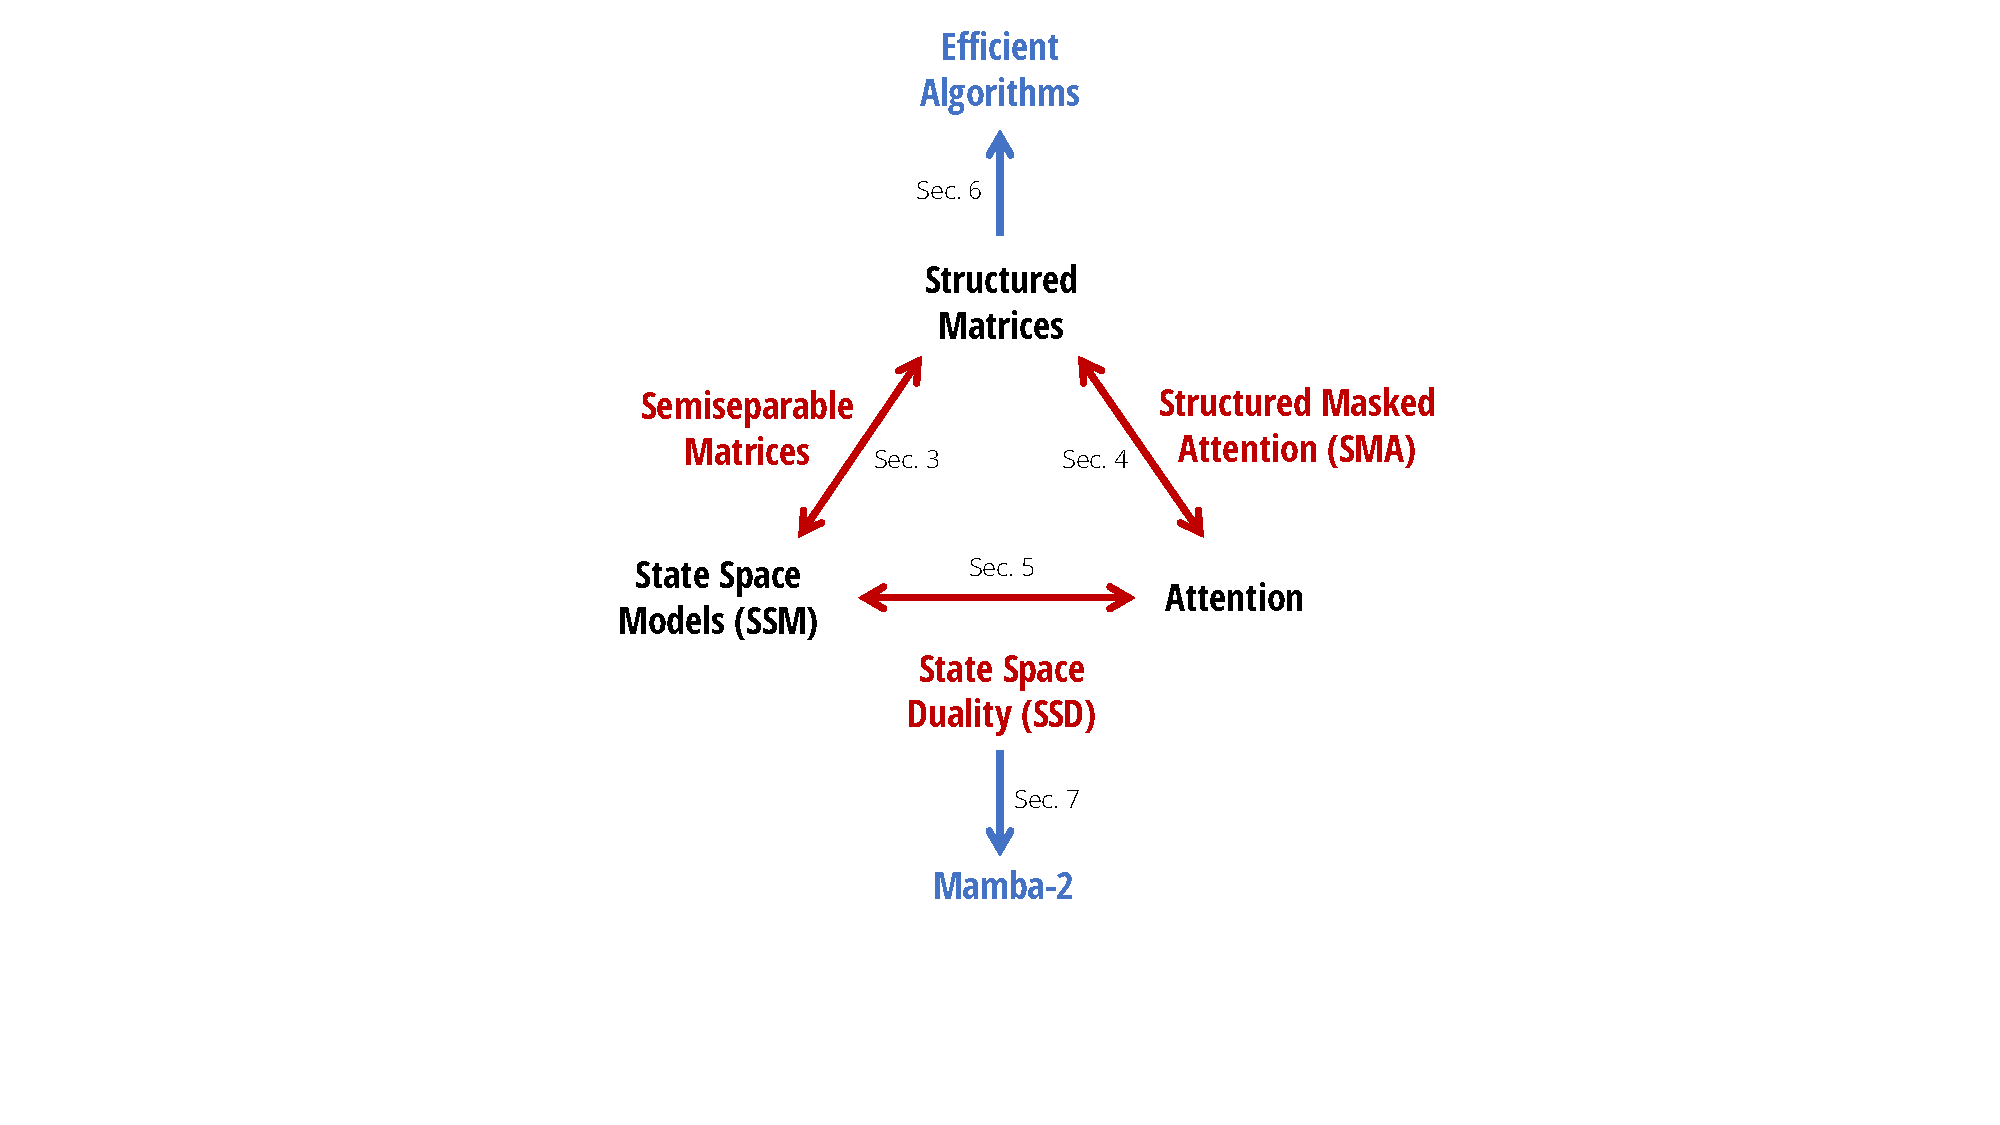
\includegraphics[width=\linewidth]{fig/ssd_roadmap.pdf}
  \end{center}
  \caption{
    (\textbf{Structured State-Space Duality}.)
    This paper fleshes out the relationship between state space models and attention through the bridge of structured matrices.
  }
  \label{fig:roadmap}
\end{wrapfigure}
}{}

\para{State Space Duality.}
Our framework connecting structured SSMs and variants of attention, which we call \textbf{structured state space duality} (SSD),
is made through the abstractions of \textbf{structured matrices}:
matrices with subquadratic parameters and multiplication complexity.
We develop two broad frameworks for representing sequence models, one as matrix transformations and one as tensor contractions, which each reveal different perspectives of the duality.
Our technical contributions include:
\begin{itemize}[leftmargin=*,itemsep=0pt,topsep=0pt]
  \item We show an equivalence between state space models and a well-studied family of structured matrices called \textbf{semiseparable matrices}\iftoggle{arxiv}{ (\cref{sec:ssm})}{}.
    This connection is at the heart our framework, revealing new properties and algorithms for SSMs. A central message of this paper is that \emph{different methods of computing state space models can be reframed as various matrix multiplication algorithms on structured matrices}.
  \item We significantly improve the theory of linear attention~\citep{katharopoulos2020transformers}.
    We first provide an incisive proof of its recurrent form through the language of tensor contractions, and then generalize it to a new family of \textbf{structured masked attention (SMA)}\iftoggle{arxiv}{ (\cref{sec:attention})}{}.
  \item We connect SSMs and SMA, showing that they have a large intersection that are duals of each other, possessing both SSM-like linear and attention-like quadratic forms\iftoggle{arxiv}{ (\cref{sec:ssd})}{}.
    \iftoggle{arxiv}{We also prove that any kernel attention method possessing a fast recurrent form must be an SSM.}{}
\end{itemize}


Beyond its intrinsic theoretical value, our framework opens up a broad set of directions for understanding and improving sequence models.

\para{Efficient Algorithms.}
First and most importantly, our framework exposes new efficient and easily-implementable algorithms for computing SSMs\iftoggle{arxiv}{ (\cref{sec:efficient})}{}.
We introduce a new \textbf{SSD algorithm}, based on block decompositions of semiseparable matrices, that takes advantage of both the linear SSM recurrence and quadratic dual form, obtaining optimal tradeoffs on all main efficiency axes (e.g. training and inference compute, memory usage, and ability to leverage matrix multiplication units on modern hardware).
A dedicated implementation of SSD is $2-8\times$ faster than the optimized selective scan implementation of Mamba, while simultaneously allowing for much larger recurrent state sizes ($8\times$ the size of Mamba or even higher, with minimal slowdown).
SSD is highly competitive with optimized implementations of softmax attention (FlashAttention-2~\citep{dao2023flashattention2}), crossing over at sequence length 2K and 6$\times$ faster at sequence length 16K.


\iftoggle{arxiv}{
\para{Architecture Design.}
One major obstacle to adopting new architectures such as SSMs is the ecosystem tailored to Transformers, such as hardware-efficient optimization and parallelism techniques for large-scale training.
Our framework allows using established conventions and techniques for attention to build a vocabulary of architecture design choices for SSMs, and further improve them (\cref{sec:architecture}).
For example, we introduce the analog of heads from multi-head attention (MHA) to SSMs.
We show that the Mamba architecture is a \textbf{multi-input SSM (MIS)} that turns out to be analogous to \textbf{multi-value attention (MVA)}, and compare other variants of Mamba with different head structures.

We also use these ideas to make slight modifications to the Mamba block, which allows tensor parallelism to be implemented (e.g. in the style of Megatron~\citep{shoeybi2019megatron}).
The main ideas include introducing grouped-value attention (GVA) head structure, and moving all data-dependent projections to occur in parallel at the beginning of the block.


}{
  \para{Mamba-2.}
  Additionally, inspired by the connection between SSMs and Transformers, we slightly modify the neural network architecture of Mamba by moving all data-dependent projections to occur in parallel at the beginning of the block. %
}
The combination of the modified parallel Mamba block, together with using SSD as the inner SSM layer, results in the \textbf{Mamba-2} architecture.
We investigate Chinchilla scaling laws for Mamba-2 in the same setting as Mamba, finding that it Pareto dominates Mamba and Transformer++ in both perplexity and wall-clock time.
We additionally train a family of Mamba-2 models at varying sizes on the Pile, showing that it matches or outperforms Mamba and open source Transformers on standard downstream evaluations.
For example, Mamba-2 with 2.7B parameters trained on 300B tokens on the Pile outperforms Mamba-2.8B, Pythia-2.8B and even Pythia-6.9B trained on the same dataset.

\iftoggle{arxiv}{
\paragraph{Systems Optimizations.}
The SSD framework connects SSMs and Transformers, allowing us to leverage a rich body of work on systems optimizations developed for Transformers~(\cref{sec:systems}).
\begin{itemize}[leftmargin=*,itemsep=0pt,topsep=0pt]
  \item For example, Tensor Parallelism (TP) is an important model parallelism technique to train large Transformer models by splitting each layer across GPUs on the same node.
    We design Mamba-2 to be TP-friendly, reducing the number of synchronization point per block by half.
  \item For very long sequences whose activations do not fit on one device, sequence parallelism has been developed for the attention blocks.
    We describe how to train SSMs in general and Mamba-2 in particular with sequence parallelism, by passing the recurrent states between devices.
  \item For finetuning with examples of different lengths, for best efficiency, Transformer requires sophisticated techniques to remove padding tokens and perform attention on variable length sequences.
    We show how Mamba-2 can be trained with variable sequence lengths efficiently, requiring no padding tokens.
\end{itemize}
}{}

\cref{sec:experiments} empirically validates Mamba-2 on language modeling, training efficiency, and a difficult multi-query associative recall task~\citep{arora2024simple}.
Finally, in \cref{sec:related}, we provide an extended related work and discuss potential research directions opened up by our framework.

Model code and pre-trained checkpoints are open-sourced at \url{https://github.com/state-spaces/mamba}.






\section{Preliminaries}
\label{sec:l2cpcc}
In this section, we first provide a background of structured representation learning and then discuss the limited representation capacity of the Euclidean space for hierarchical information, which serves as the primary motivation for our work. 

\subsection{Background}

Structured representation learning \citep{zeng2022learning} breaks the permutation invariance of flat representation learning by incorporating a hierarchical regularization term with a standard classification loss. The regularization term is specifically designed to enforce class-conditioned grouping or partitioning in the feature space, based on a given hierarchy.

More specifically, given a weighted tree $\mathcal{T} = (V, E, e)$ with vertices $V$, edges $E$ and edge weights $e$, let us compute a tree metric $d_\mathcal{T}$ for any pair of nodes $v,v' \in V$, as the weighted length of the shortest path in $\mathcal{T}$ between $v$ and $v'$. For a real world dataset $\data = \{(\vx_i, y_i)\}_{i = 1}^N$, we can specify a \emph{label tree} $\mathcal{T}$ where a node $v_i\in V$,  $v_i$ corresponds to a subset of classes, and $\data_i\subseteq \data$ denote the subset of data points with class label $v_i$. We denote dataset distance between $\data_i$ and $\data_j$ as $\rho(v_i, v_j) = d\left(\data_i,\data_j\right)$, where $d(\cdot, \cdot)$ is any distance metric in the feature space, varied by design.

With a collection of tree metric $d_\mathcal{T}$ and dataset distances $\rho$, we can use the Cophenetic Correlation Coefficient (CPCC) \citep{cpcc}, inherently a Pearson's correlation coefficient, to evaluate the correspondence between the nodes of the tree, and the features in the representation space. Let $\overline{d_\mathcal{T}}, \overline{\rho}$ denote the mean of the collection of distances, then CPCC is defined as
\begin{equation}
\label{eq:CPCC}
    \cpcc(d_\mathcal{T}, \rho) := \frac{\sum_{i<j}(d_\mathcal{T}(v_i,v_j) - \overline{d_\mathcal{T}})(\rho(v_i,v_j) - \overline{\rho})}{(\sum_{i<j}(d_\mathcal{T}(v_i,v_j) - \overline{d_\mathcal{T}})^2)^{1/2} (\sum_{i<j}(\rho(v_i,v_j) - \overline{\rho})^2)^{1/2}}. 
\end{equation}
For the supervised classification task, we consider the training set  $\mathcal{D}_{\text{tr}}^{\text{in}} = \{(\vx_i, y_i)\}_{i=1}^N$ and we aim to learn the network parameter $\theta$ for a feature encoder $f_\theta : \mathcal{X} \to \gZ$, where $\gZ \subseteq \mathbb{R}^{d}$ denotes the representation/feature space. For structured representation learning, the feature encoder is usually followed by a classifier $g_{w}$, and the parameters $\theta, w$ are learnt by minimizing $\gL$ along with a standard \emph{flat} (non-hierarchical) classification loss, for instance, Cross-Entropy (\texttt{CE}) or Supervised Contrastive (\texttt{SupCon}) \citep{2020supcon} loss, with the structured regularization term as:
\begin{equation}
    \label{eq:objective_regularizer}
    \mathcal{L}(\data) = \sum_{(\vx, y)\in \data} \ell_\text{Flat}(\vx,y,\theta, w) - \alpha\cdot\cpcc(\tmetric, \rho).        
\end{equation}
Using a composite objective as defined in~\Cref{eq:objective_regularizer}, we can enforce the distance relationship between a pair of representations in the feature space, to behave similarly to the tree metric between the same vertices. For instance, consider a simple label tree with a root node, a coarse level, and a fine level, where subsets of fine classes share the same coarse parent. For this hierarchy, we would expect the fine classes of the same parents (e.g., \emph{apple} and \emph{banana} are \emph{fruits}) to have closer representations in the feature space, whereas fine classes with different coarse parents (e.g., an \emph{apple} is a \emph{fruit} and a \emph{tulip} is a \emph{flower}) should be further apart. The learned structure-informed representations reflect these hierarchical relationships and lead to interpretable features with better generalization \citep{zeng2022learning}.

\subsection{$\ell_2$-CPCC}

\Cref{eq:CPCC} offers the flexibility of designing a metric to measure the similarity between two data subsets, and \citet{zeng2022learning} define the \emph{Euclidean dataset distance} as $\rho_{\ell_2}(\data_i, \data_j) := \|\frac{1}{|\data_i|}\sum_{\vx\in \data_i}f(\vx) - \frac{1}{|\data_j|}\sum_{\vx'\in \data_j}f(\vx')\|_2$. The distance between datasets is thus the $\ell_2$ distance between two Euclidean \emph{centroids} of their class-conditioned representations, which is unsuitable for modeling \emph{tree-like} data \citep{chen2013hyperbolicity}. 
Additionally, this regularization approach in \citet{zeng2022learning} is applied only to the leaf nodes of $\mathcal{T}$ for efficiency.

However, this leaf-only formulation of the CPCC offers an \emph{approximation} of the structured information, since the distance between non-leaf nodes is not restricted explicitly by the regularization. This approximation, therefore, leads to a loss of information contained in the original hierarchy $\mathcal{T}$.

Actually, it is impossible to embed $d_\mathcal{T}$ into $\ell_2$ exactly. Or more formally, there exists no bijection $\varphi$ such that $d_\mathcal{T}(\varphi(\vz_i), \varphi(\vz_j)) = \lVert \vz_i - \vz_j \rVert_2$ irrespective of how large the feature dimension $d$ is. We provide two such examples for a toy label tree in \Cref{fig:failure}, below. 

\begin{wrapfigure}{l}{0.4\textwidth}
\centering
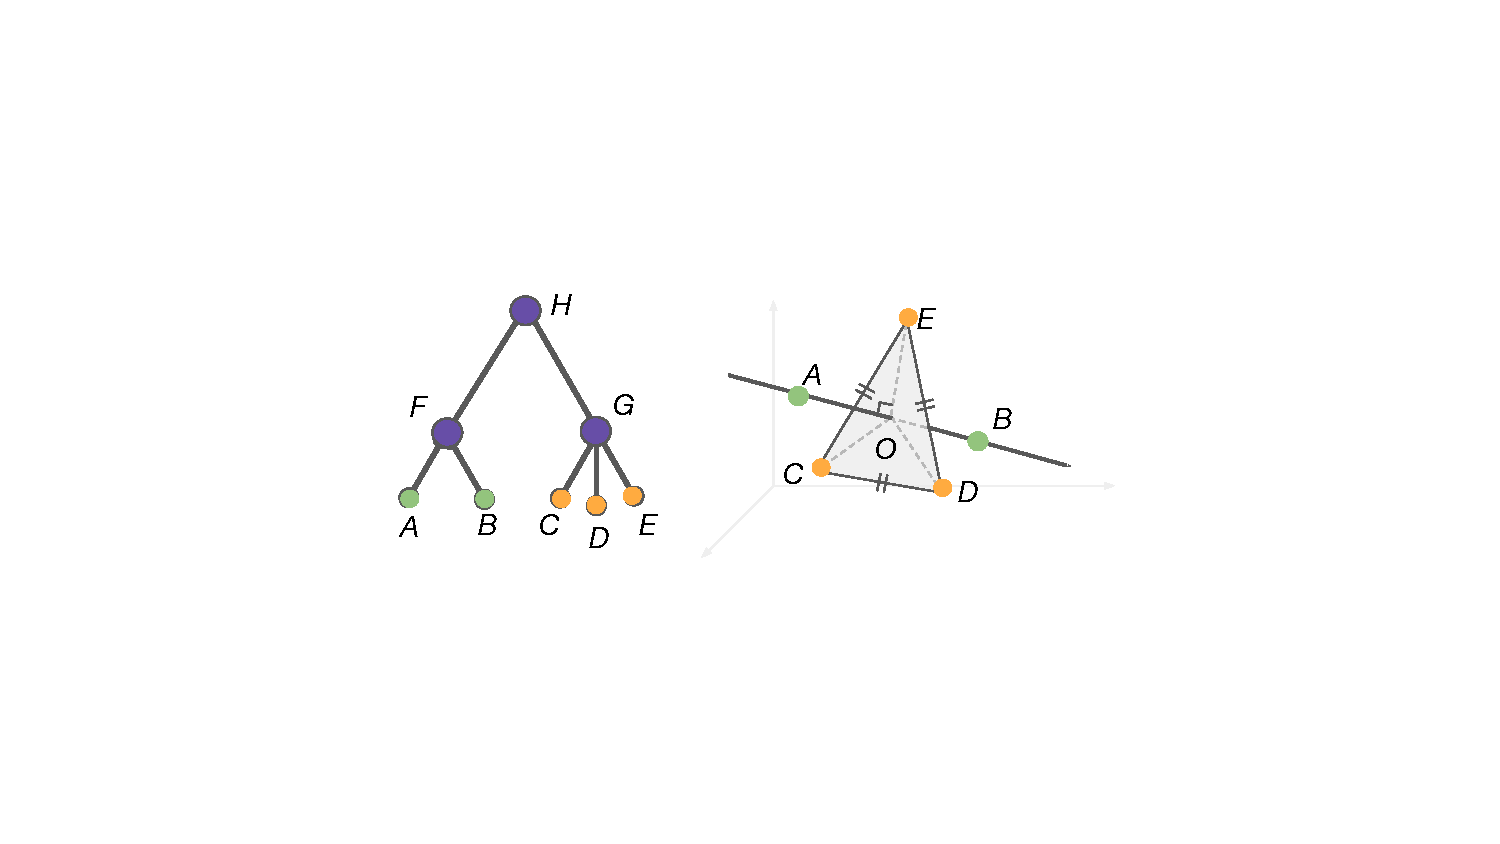
\includegraphics[width=\linewidth]{figures/l2_failure.pdf}\hspace*{-0.4cm}
\caption{(left) An unweighted label tree with two coarse nodes: $F$, $G$. $F$ contains two fine classes $A,B$ and $G$ contains three fine classes $C,D,E$. We cannot embed this in $\ell_2$ exactly (right).}
\vspace{-1em}
\label{fig:failure}
\end{wrapfigure}

\textbf{Example 1.} We intend to embed all nodes in $\gT$, including purple internal nodes. Notice that $G,C,D,E$ is a star graph centered at $G$. Since $CG = DG = 1, CD = 2$, by triangle inequality $C,D,G$ must be on the same line where $G$ is the center of $CD$. Similarly, $G$ must be at the center of $DE$. Hence, the location of $E$ must be at $C$, which contradicts the uniqueness of all nodes in $\gT$.

\textbf{Example 2.} As an easier problem, let us only embed leaf nodes into the Euclidean space as shown in \Cref{fig:failure}. Since $CD = DE = CE = 2$, they must be on a plane with an equilateral triangle $\triangle_{CDE}$ in Euclidean geometry. Then all the green classes have the same distance $4$ to each yellow class. Therefore, $A,B$ must be on the line perpendicular to $\triangle_{CDE}$ and intersecting the plane with $O$, which is the barycenter of $\triangle_{CDE}$. Due to the uniqueness and symmetry of $A,B$, we must have $AO = BO = 1$ to satisfy $AB = 2$. $AO = 1, OE = \frac{2\sqrt{3}}{3}, AE = 4$ which contradicts the Pythagorean Theorem.

\begin{figure}[t]
\vspace{-1em}
\centering
\begin{subfigure}{.5\textwidth}
  \centering
  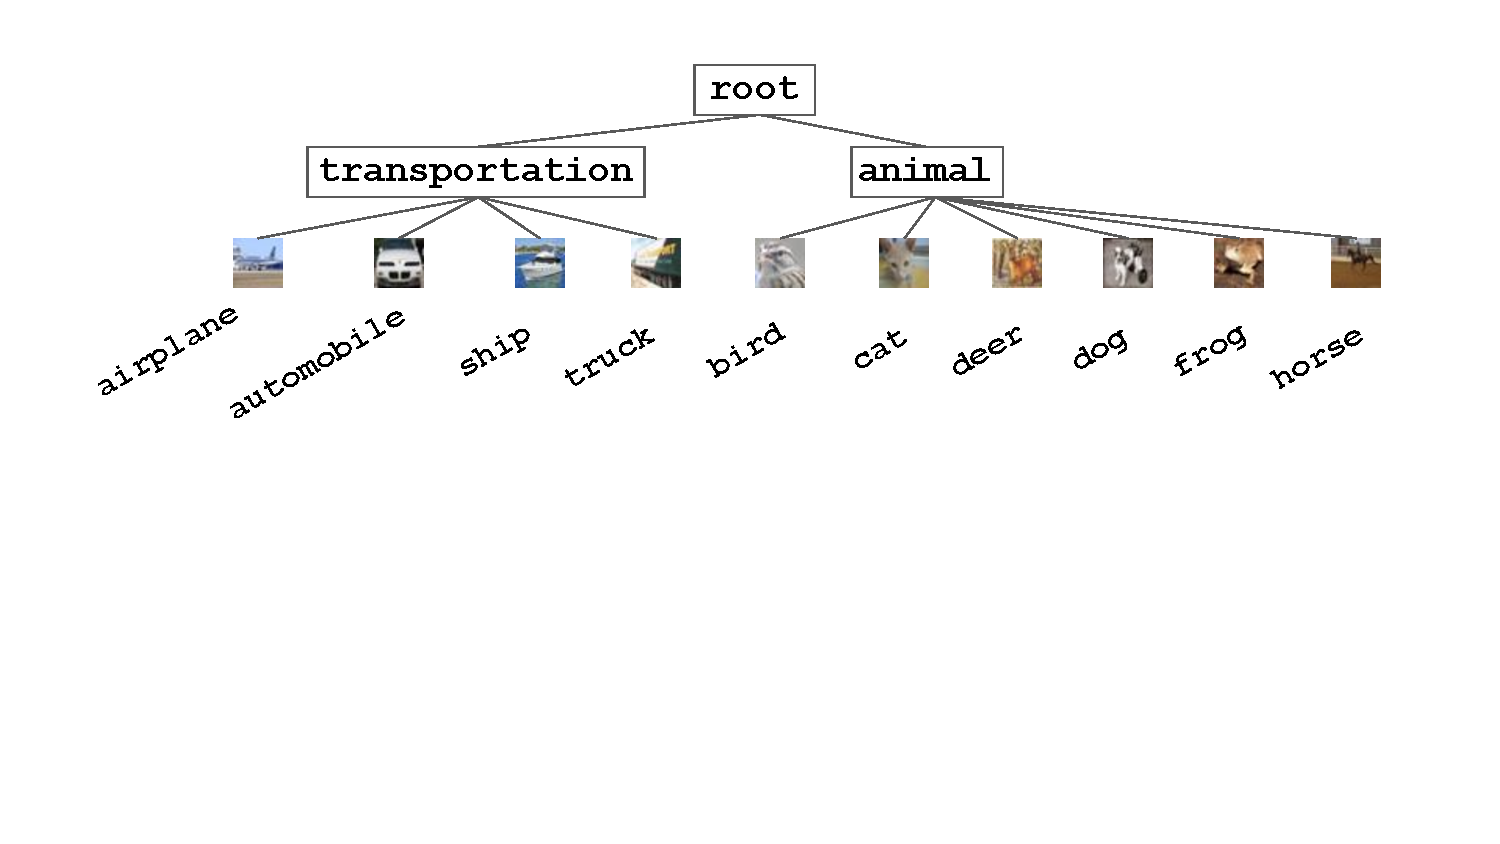
\includegraphics[width=\linewidth]{figures/CIFAR10Tree.pdf}
\end{subfigure}%
\begin{subfigure}{.5\textwidth}
  \centering
  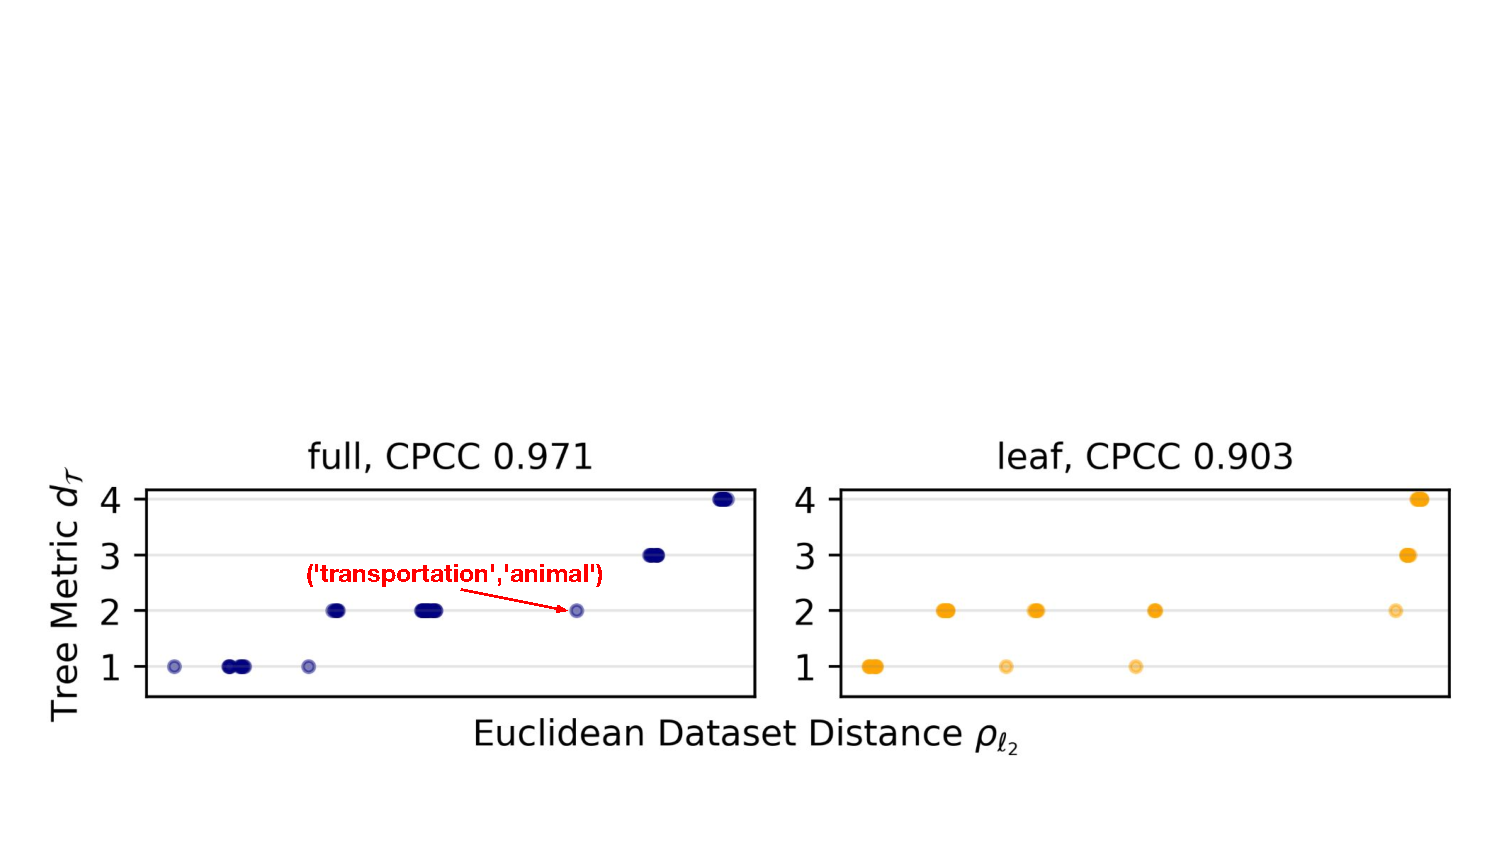
\includegraphics[width=\linewidth]{figures/CIFAR10CPCC.pdf}
\end{subfigure}
\caption{Using $\ell_2$-CPCC for structured representation on CIFAR10. CIFAR10 hierarchy (left) has a three level structure with $13$ vertices. For a $512$-dimensional embedding, we apply $\ell_2$-CPCC either for the full tree (middle) or the leaf nodes only (right) and plot the ground truth tree metric against pairwise Euclidean centroid distances of the learnt representation. The optimal train CPCC is $1$.}
\vspace{-1em}
\label{fig:toy}
\end{figure}

Since we cannot embed an arbitrary tree $\gT$ into $\ell_2$ without distortion, it would also affect the optimization of the $\ell_2$-CPCC in a classification problem, where the tree weights encode knowledge of class similarity. To verify our claims, we consider the optimization of $512$-dimensional $\ell_2$-CPCC structured representations for CIFAR10 \citep{krizhevsky2009learning}. The CIFAR10 dataset consists of a small label hierarchy as shown in \Cref{fig:toy} (left). 

The optimal CPCC is achieved when each tree metric value corresponds to a single $\rho_{\ell_2}$. However, in \Cref{fig:toy} (right), even with an optimization of the $\ell_2$-CPCC loss for the entire tree, we observe a sub-optimal train CPCC less than $1$, where the distance between two coarse nodes, \emph{transportation} and \emph{animal}, is far away from the desired solution. Furthermore, optimization of the CPCC loss for only the leaf nodes, leads to an even larger distortion of the tree metrics. 


\section{Methodology}
\label{sec:methodology}

Hyperbolic spaces are more suitable for embedding hierarchical relationships with low distortion \citep{Sarkar_2012} and low dimensions. Hence, motivated by the aforementioned challenges, we propose a \textbf{Hyp}erbolic \textbf{Structure}d regularizer for \emph{hierarchy-informed} representation learning. We begin with the basics of hyperbolic geometry, followed by the detailed methodology of our proposed approach.

\subsection{Hyperbolic Geometry}
\begin{wrapfigure}{r}{0.3\textwidth}
\centering
\vspace{-1em}
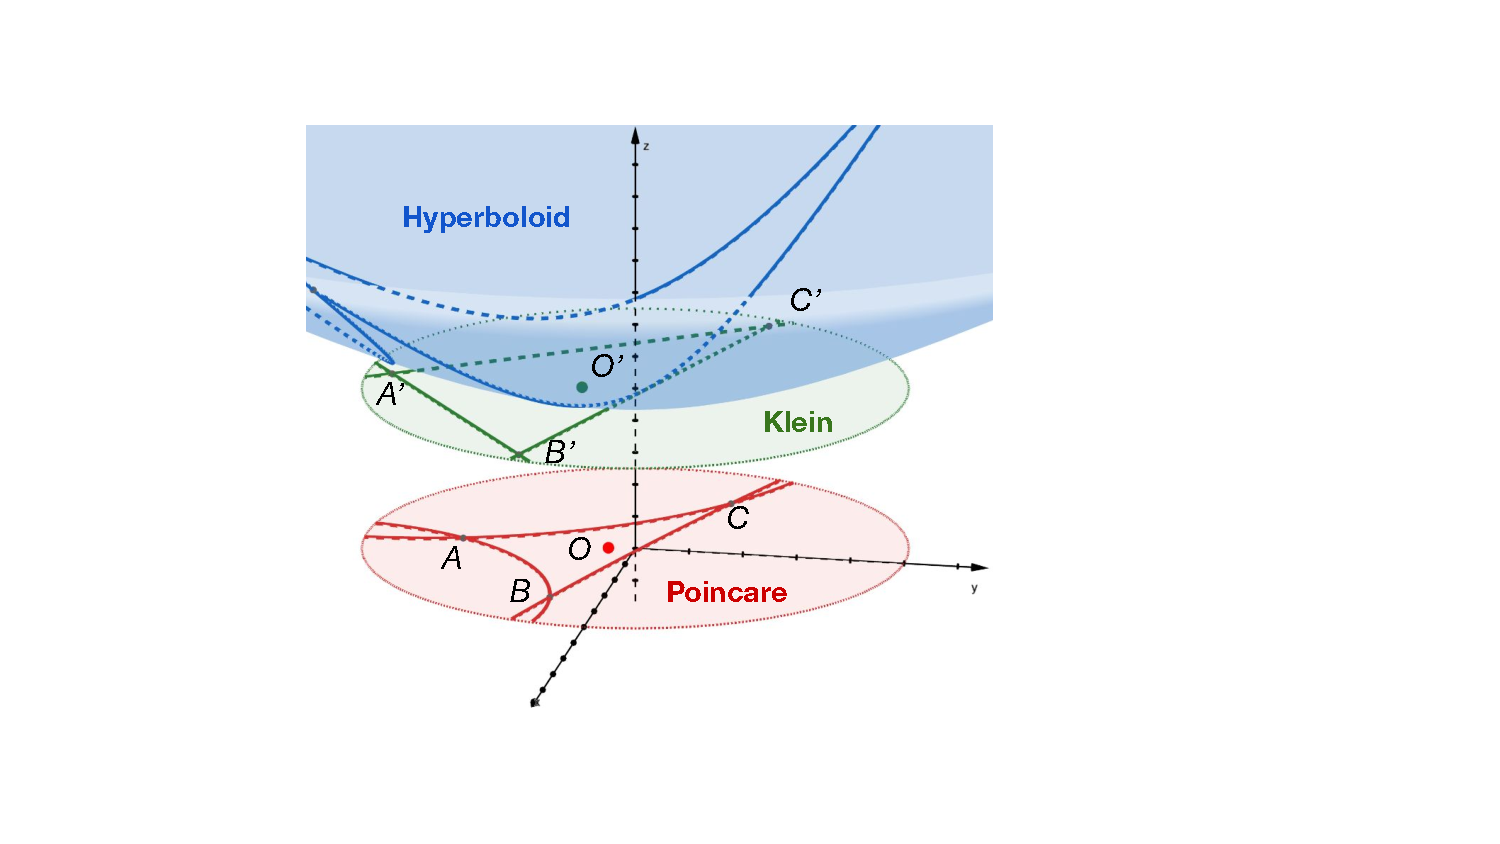
\includegraphics[width=.95\linewidth]{figures/hyperbolic.pdf}
\caption{Lines on different models for $2$-dimensional hyperbolic space.}
\vspace{-1em}
\label{fig:hyperbolic_models}
\end{wrapfigure}

Hyperbolic spaces are non-Euclidean spaces with negative curvature where given a fixed point and a line, there exist infinitely many parallel lines that can pass through this point. There are several commonly used isometric hyperbolic models \citep{cannon1997hyperbolic}. For this work, we mainly use the Poincaré Ball model. 

\begin{definition}[Manifold]
\label{eq:manifold}
A \textit{manifold} $\gM$ is a set of points $\vz$ that are locally Euclidean. Every point $\vz$ of the manifold $\gM$ is attached to a \textit{tangent space} $\gT_\vz \gM$, which is a vector space over the reals of the same dimensionality as $\gM$ that contain all the possible directions that can tangentially pass through $\vz$.
\end{definition}

\begin{definition}[\Poincare Ball Model] Given $c$ as a constant, the \Poincare ball model $(\sB_c^d,\mathfrak{g}_B)$ is defined by a manifold of an open ball $\sB_c^d=\{\vz\in\sR^d:c\|\vz\|^2< 1\}$ and metric tensor $\mathfrak{g}_B$ that defines an inner product of $\gT_\vz \sB_c^d$. The model is equipped with the distance \citep{ungar2001hyperbolic} as
\begin{equation}
d_{\sB_c}(\vz_1,\vz_2) = \frac{2}{\sqrt{c}}\tanh^{-1}\left(\sqrt{c}\left\lVert\frac{-(1 + 2c\left<-\vz_1, \vz_2\right> + c\|\vz_2\|^2)\vz_1 + (1 - c\|\vz_1\|^2)\vz_2}{1 - 2c\left<\vz_1,\vz_2\right> + c^2\|\vz_1\|^2\|\vz_2\|^2}\right\rVert\right).
\label{eq:poincaredistance}
\end{equation}
\end{definition}
For $c \to 0$, we can recover the properties of the Euclidean geometry since $\lim_{c \to 0} d_{\sB_c}(\vz_1,\vz_2) = 2\|\vz_1-\vz_2\|$. Since $\gT_\vz \sB_c^d$ is isomorphic to $\mathbb{R}^d$, we can connect vectors in Euclidean space and hyperbolic space with the bijection between $\gT_\vz \sB_c^d$ and $\sB_c^d$ \citep{ungar2001hyperbolic}. For $\vz = \mathbf{0}$, the \emph{exponential map} $\exp_\mathbf{0}^c : \gT_\vz \sB_c^d \to \sB_c^d$ and \emph{logarithm map} $\log_\mathbf{0}^c : \sB_c^d \to \gT_\vz \sB_c^d$ have the closed form of
\begin{equation}
\label{eq:hyp_maps}
    \exp_\mathbf{0}^c (\vv) = \tanh\left(\sqrt{c} \|\vv\| \right)\frac{\vv}{\sqrt{c}\|\vv\|}, \quad \log_\mathbf{0}^c (\vu) = \frac{1}{\sqrt{c}}\tanh^{-1}\left(\sqrt{c} \| \vu \| \right)\frac{\vu}{\|\vu \|}. 
\end{equation}
Alternatively, to guarantee the correctness of Poincaré distance computation, we can also process any Euclidean vector with a clipping module \citep{nickel2017poincare}
\begin{equation}
    \text{clip}^c(\vv) = \begin{cases}
			\vv, & \text{if $\|\vv\|< 1 / \sqrt{c}$}\\
                \left(\frac{1}{\sqrt{c}} - \epsilon\right) \frac{\vv}{\|\vv\|} , & \text{otherwise}
		 \end{cases},
\end{equation}
so the clipped vector is within the Poincare disk. We set $\epsilon$ as a small positive number in practice.

\begin{definition}[Klein Model]
Klein model $(\mathbb{K}_c^d, \mathfrak{g}_K)$ consists of an $1/\sqrt{c}$-radius open ball $\mathbb{K}_c^d = \{\vz\in\sR^d:c\|\vz\|^2 < 1\}$ and a metric tensor $\mathfrak{g}_K$ different from $\mathfrak{g}_B$. Similar to the mean computation in Euclidean space, let $\gamma_i = 1 / \sqrt{1 - c\|\vz_i\|^2}$, the Einstein midpoint of a group of Klein vectors $\vz_1, \dots \vz_n \in \mathbb{K}_c^d$ has a simple expression of a weighted average
\begin{equation}
    \text{HypAve}_K(\vz_1, \dots \vz_n) = \sum\limits_{i=1}^n \gamma_i \vz_i \bigg/ \sum\limits_{i=1}^n \gamma_i.
    \label{eq:hypave}
\end{equation}
\end{definition}
We illustrate the relationship between the different hyperbolic models in \Cref{fig:hyperbolic_models}. The hyperboloid space models $d$-dimensional hyperbolic geometry on a $d+1$-dimensional space. When $d = 2$, the Klein model is the tangent plane of the hyperboloid model at $(0,0,1)$, and the \Poincare disk shares the same support as the Klein disk, although shifted downwards and centered at the origin. Given a triangle on the hyperboloid model, its projection on the Klein model preserves the straight sides, but the projection of a line on the \Poincare model is a part of a circular arc or the diameter of the disk. Let $\vz_\mathbb{B}, \vz_\mathbb{K}$ be coordinates of $\vz$ under \Poincare and Klein model respectively, the prototype operations on $\mathbb{B}^d_c$ require transformations between $\mathbb{B}^d_c$ and $\mathbb{K}^d_c$ as
\begin{equation}
    \vz_\mathbb{B} = \frac{\vz_\mathbb{K}}{1 + \sqrt{1 - c\|\vz_\mathbb{K}\|^2}}, \quad \vz_\mathbb{K} = \frac{2\vz_\mathbb{B}}{1 + c\|\vz_\mathbb{B}\|^2}.
    \label{eq:Poincare2Klein}
\end{equation}
For example, in \Cref{fig:hyperbolic_models}, $O'$ is the $\text{HypAve}_\text{K}$ of $A',B',C'$, and can be mapped back to the \Poincare disk to get the \Poincare prototype ($\text{HypAve}_\text{B}$) $O$ of points $A, B, C$ by a change of coordinates.

\subsection{\texttt{HypStructure}: Hyperbolic Structured Regularization}
\label{sec:hypstructure-method}
At a high level, \texttt{HypStructure} uses a combination of two losses: a Hyperbolic Cophenetic Correlation Coefficient Loss (\texttt{HypCPCC})), and a Hyperbolic centering loss (\texttt{HypCenter}) for embedding the hierarchy in the representation space. Below we describe the two components of \texttt{HypStructure}. The pseudocode of \texttt{HypStructure} is shown in \Cref{alg:hypstructure} in \Cref{app:pseudocode}.


\textbf{HypCPCC (\underline{Hyp}erbolic \underline{C}o\underline{p}henetic \underline{C}orrelation \underline{C}oefficient):} We extend the $\ell_2$-CPCC methodology in \citet{zeng2022learning} to the hyperbolic space in \texttt{HypCPCC}. Three major steps of \texttt{HypCPCC} are (i) map Euclidean vectors to \Poincare space (ii)  compute class prototypes  (iii) use \Poincare distance for CPCC. Specifically, we first project each $\vz_i \in \mathbb{R}^d$ to $\mathbb{B}_c^d$, and compute the Poincaré centroid for each vertex of $\mathcal{T}$ using hyperbolic averaging as shown in \Cref{eq:hypave} and \Cref{eq:Poincare2Klein}. Alternatively, we can also compute Euclidean centroids $\overline{\vz} = \frac{1}{|\data_i|}\sum_{\vz \in \data_i}{\vz}$ for each vertex, and project each $\overline{\vz} \in \mathbb{R}^d$ to $\mathbb{B}_c^d$ either by $\exp_{\mathbf{0}}^c$ or $\text{clip}^c$. After the computation of hyperbolic centroids, we use the pairwise distances between all vertex pairs in $\mathcal{T}$ in the \Poincare ball, to compute the \texttt{HypCPCC} loss using \Cref{eq:CPCC} by setting $\rho = d_{\mathbb{B}_c}$. 

\textbf{HypCenter (\underline{Hyp}erbolic \underline{Center}ing):} Inspired by Sarkar's low-distortion construction \citep{Sarkar_2012} that places the root node of a tree at the origin, we propose a centering loss for this positioning, that enforces the representation of the root node to be close to the center of the \Poincare disk, and the representations of its children to be closer to the border of \Poincare disk. We enforce this constraint by minimizing the norm of the hyperbolic representation of the root node as $\ell_\text{center} = \norm{\text{HypAve}_B(\exp_{\mathbf{0}}^c(\vz_1), \dots, \exp_{\mathbf{0}}^c(\vz_N))}$. Alternatively, for centroids computed in the Euclidean space and mapped to the \Poincare disk, we minimize $\ell_\text{center} = \norm{1/N\sum_{i=1}^N f_\theta(\vx_i)}$ directly due to the monotonicity of $\tanh(\cdot)$ in the exponential map.

Finally, for $\alpha, \beta > 0$, we can learn the \emph{hierarchy-informed} representations by minimizing
\begin{equation}
    \label{eq:objective_hyp}
    \mathcal{L}(\data) = \sum_{(\vx, y)\in \data} \ell_\text{Flat}(\vx,y,\theta) - \alpha\cdot\hypcpcc(\tmetric, d_{\mathbb{B}_c}) + \beta \cdot\ell_\text{center}(\vx, \theta),
\end{equation}
where $\ell_\text{Flat}$ is a standard classification loss, such as the \texttt{CE} loss or the \texttt{SupCon} loss. 



\textbf{Time Complexity:} In a batch computation setting with a batch size $b$ and the number of classes (leaf nodes) as $k$, the computational complexity for a \texttt{HypStructure} computation to embed the full tree will still be $O(d\cdot\min\{b^2,k^2\})$, which is the same as the complexity of a Euclidean \emph{leaf-only} CPCC. The additional knowledge gained from internal nodes allows us to reason about the relationship between higher-level  concepts, and the hyperbolic representations help in achieving a low distortion of hierarchical information for better performance in downstream tasks.

\vspace{-0.2cm}
\section{Experiments Details}
\label{sec:exp}

\vspace{-0.2cm}
\subsection{Roadmap Insights on FFHQ-256\texorpdfstring{~\cite{sg1}}{}}
\label{sub:arc-experiments}
\vspace{-0.1cm}
As per Table~\ref{tab:roadmap}, Config A (vanilla StyleGAN2) achieves an FID of 7.52 using the official implementation on FFHQ-256. Config B with all tricks removed achieves an FID of 12.46---performance drops as expected. 
Config C, with a well-behaved loss, achieves an FID of 11.65. But, now training is sufficiently stable to improve the architecture.

Config D, which improves $G$ and $D$ based on the classic ResNet and ConvNeXt findings, achieves an FID of 9.95. The output skips of the StyleGAN2 generator are no longer useful given our new architecture; including them produces a worse FID of 10.17. Karras~\etal find that the benefit of output skips is mostly related to gradient magnitude dynamics~\cite{sg3}, and this has been addressed by our ResNet architecture. For StyleGAN2, Karras~\etal conclude that a ResNet architecture is harmful to $G$~\cite{sg2}, but this is not true in our case as their ResNet implementation is considerably different from ours: 1) Karras~\etal use one 3-3 residual block for each resolution stage, while we have a separate transition layer and two 1-3-1 residual blocks; 2) i.3) and i.4) are violated as they do not have a linear residual block~\cite{mobnet} and the transition layer is placed on the skip branch of the residual block rather than the stem; 3) the essential principle of ResNet~\cite{resnet}---identity mapping~\cite{resnet2}---is violated as Karras~\etal divide the output of the residual block by $\sqrt{2}$ to avoid variance explosion due to the absence of a proper initialization scheme.

For Config E, we conduct two experiments that ablate i.\ref{item:i1} (increased width with depthwise conv.) and i.\ref{item:i2} (an inverted bottleneck). We add GroupedConv and reduce the bottleneck compression ratio to two given the same model size. Each bottleneck is now 1.5$\times$ the width of Config A, and the FID drops to 7.51, surpassing the performance of StyleGAN2. By inverting the stem and the bottleneck dimensions to enhance the capacity of GroupedConv, our final model achieves an FID of 7.05, exceeding StyleGAN2.


\begin{wraptable}[12]{r}{6.5cm}
\vspace{-1.25cm}
\centering
\caption{StackedMNIST 1000-mode coverage.}
% Our model outperforms other GANs in terms of $D_\text{KL}$, indicating that we are better able to recover the distribution.}
\vspace{-0.4cm}
\resizebox{0.8\linewidth}{!}{
\begin{tblr}{
  cell{2}{2} = {c},
  cell{2}{3} = {c},
  cell{3}{2} = {c},
  cell{3}{3} = {c},
  cell{4}{2} = {c},
  cell{4}{3} = {c},
  cell{5}{2} = {c},
  cell{5}{3} = {c},
  cell{6}{2} = {c},
  cell{6}{3} = {c},
  cell{7}{2} = {c},
  cell{7}{3} = {c},
  cell{8}{2} = {c},
  cell{8}{3} = {c},
  cell{9}{2} = {c},
  cell{9}{3} = {c},
  cell{10}{2} = {c},
  cell{10}{3} = {c},
  cell{11}{2} = {c},
  cell{11}{3} = {c},
  cell{12}{2} = {c},
  cell{12}{3} = {c},
  hline{2,12} = {1-3}{},
}
Model     & \# modes$\uparrow$ & $D_\text{KL}$$\downarrow$            &  \\
DCGAN~\cite{dcgan}     & 99            & 3.40\phantom{0}&  \\
VEEGAN~\cite{srivastava2017veegan}    & 150           & 2.95\phantom{0}&  \\
WGAN-GP~\cite{wgan-gp}& 959           & 0.73\phantom{0}&  \\
PacGAN~\cite{pacgan}    & 992           & 0.28\phantom{0}&  \\
StyleGAN2~\cite{sg2} & 940           & 0.42\phantom{0}&  \\
PresGAN~\cite{presgan}   & \textbf{1000} & 0.12\phantom{0}&  \\
Adv. DSM~\cite{advsm}  & \textbf{1000} & 1.49\phantom{0}&  \\
VAEBM~\cite{vaebm}     & \textbf{1000} & 0.087          &  \\
DDGAN~\cite{ddgan}     & \textbf{1000} & 0.071          &  \\
MEG~\cite{meg}       & \textbf{1000} & 0.031          &  \\
Ours---Config E     & \textbf{1000} & \textbf{0.029} &  
\end{tblr}
}
\label{tab:stackedmnist}
\end{wraptable}%

\subsection{Mode Recovery --- StackedMNIST\texorpdfstring{~\cite{metz2016unrolled}}{}} 
\vspace{-0.1cm}
We repeat the earlier experiment in 1000-mode convergence on StackedMNIST (unconditional generation), but this time with our updated architecture and with comparisons to SOTA GANs and likelihood-based methods (Tab.~\ref{tab:stackedmnist}, Fig.~\ref{fig:stacked-mnist}). 
One advantage brought up of likelihood-based models such as diffusion over GANs is that they achieve mode coverage~\cite{adm}. We find that most GANs struggle to find all modes. But, PresGAN~\cite{presgan}, DDGAN~\cite{ddgan}, and our approach are successful. Further, our method outperforms all other tested GAN models in term of KL divergence.

\subsection{FID --- FFHQ-256\texorpdfstring{~\cite{sg1}}{} (Optimized)}
\vspace{-0.1cm}
We train Config E model until convergence and with optimized hyperparameters and training schedule on FFHQ at 256$\times$256 (unconditional generation) (Tab.~\ref{tab:ffhq256}, Figs.~\ref{fig:ffhq-256-teaser} and~\ref{fig:ffhq-256}). 
Please see our supplemental material for training details.
%The hyperparameters and schedule are listed in the supplemental material. 
Our model outperforms existing StyleGAN methods, plus four more recent diffusion-based methods. On this common dataset experimental setting, many methods (not listed here) use the bCR~\cite{zhao2021improved} trick---this has only been shown to improve performance on FFHQ-256 (not even at different resolutions of FFHQ)~\cite{zhao2021improved, zhang2022styleswin}. We do not use this trick. 
% no such tricks in our method.
% JT Try to minimize embellishment...
% This is particularly impressive given the fact that the dataset FFHQ was designed for StyleGAN~\cite{sg1} and the StyleGAN series of models were optimized with this specific dataset in mind.
% to achieve this performance.

\subsection{FID --- FFHQ-64\texorpdfstring{~\cite{edm}}{}}
\vspace{-0.1cm}
To compare with EDM~\cite{edm} directly, we evaluate our model on FFHQ at 64$\times$64 resolution. For this, we remove the two highest resolution stages of our 256$\times$256 model, resulting in a generator that is less than half the number of parameters as EDM. Despite this, our model outperforms EDM on this dataset and needs one function evaluation only (Tab.~\ref{tab:ffhq64}).

\begin{figure}
\begin{floatrow}
    %\hspace{-0.75cm}%
    \capbtabbox{%
        \centering
        \resizebox{\linewidth}{!}{
        \begin{tblr}{
          column{2,3} = {r},
          cell{1}{2} = {c},
          cell{1}{3} = {c},
          hline{2,5,9,10} = {-}{},
        }
        Model       & NFE$\downarrow$ & FID$\downarrow$  \\
        StyleGAN2~\cite{sg2}   & 1               & 3.78 \\
        StyleGAN3-T~\cite{sg3} & 1               & 4.81 \\
        StyleGAN3-R~\cite{sg3} & 1               & 3.92 \\
        LDM~\cite{rombach2022high} & 200               & 4.98\\
        ADM (DDIM)~\cite{adm,compdiff} & 500               & 8.41\\
        ADM (DPM-Solver)~\cite{adm,compdiff} & 500               & 8.40\\
        Diffusion Autoencoder~\cite{diffae,compdiff} & 500               & 5.81\\
        Ours---Config E  & 1               & 2.75 \\
        \emph{With ImageNet feature leakage~\cite{kynkaanniemi2022role}:} & & \\
        PolyINR*~\cite{singh2023polynomial} & 1               & 2.72 \\
        StyleGAN-XL*~\cite{sgxl} & 1               & 2.19 \\
        StyleSAN-XL*~\cite{takida2024san} & 1               & 1.68 \\
        \end{tblr}
        }
    }{%
        \caption{
        \label{tab:ffhq256}FFHQ-256. * denotes models that leak ImageNet features.}
    }
    %
    \capbtabbox{%
        \centering
        \resizebox{0.85\linewidth}{!}{
        \begin{tblr}{
          column{2} = {r},
          column{3} = {r},
          hline{2,5,8} = {-}{},
        }
        Model         & NFE$\downarrow$ & FID$\downarrow$ \\
        StyleGAN2~\cite{sg2,anycostgan}     & 1               & 3.32            \\
        MSG-GAN~\cite{karnewar2020msg,anycostgan}       & 1               & 2.7             \\
        Anycost GAN~\cite{anycostgan}   & 1               & 2.52            \\
        VE~\cite{sde,edm}            & 79              & 25.95           \\
        VP~\cite{sde,edm}            & 79              & 3.39            \\
        EDM~\cite{edm}           & 79              & 2.39            \\
        Ours—Config E & 1               & 1.95 \\
        \end{tblr}
        }
    }{%
        \caption{\label{tab:ffhq64}FFHQ-64.}
    }
\end{floatrow}
\vspace{-0.25cm}
\end{figure}


% \begin{figure}
% \begin{floatrow}
%     \capbtabbox{%
%         \centering
%         \resizebox{0.8\linewidth}{!}{
%         \begin{tblr}{
%           column{2,3} = {r},
%           cell{1}{2} = {c},
%           cell{1}{3} = {c},
%           hline{2,9,13} = {-}{},
%         }
%         Model               & NFE$\downarrow$ & FID$\downarrow$ \\
%         BigGAN~\cite{biggan}              & 1               & 14.73 \\
%         TransGAN~\cite{trans}            & 1               & 9.26 \\
%         ViTGAN~\cite{vitgan}              & 1               & 6.66 \\
%         DDGAN~\cite{ddgan}               & 4               & 3.75 \\
%         Diffusion StyleGAN2~\cite{diffusiongan} & 1               & 3.19 \\
%         StyleGAN2 + ADA~\cite{sg2ada}     & 1               & 2.42 \\
%         StyleGAN3-R + ADA~\cite{sg3,studio}   & 1               & 10.83 \\
%         DDPM~\cite{ddpm}               & 1000            & 3.21 \\
%         DDIM~\cite{ddim}                & 50             & 4.67 \\
%         VE~\cite{sde,edm}                  & 35              & 3.11 \\
%         VP~\cite{sde,edm}                  & 35              & 2.48 \\
%         Ours---Config E     & 1               & 1.96 \\
%         \hline
%         \emph{With ImageNet feature leakage~\cite{kynkaanniemi2022role}:} & & \\
%         StyleGAN-XL*~\cite{sgxl}       & 1               & 1.85 \\
%         \end{tblr}
%         }
%     }{%
%         \caption{\label{tab:cifar10}CIFAR-10.}
%     }
%         % \begin{tblr}{
%         %   column{2,3} = {r},
%         %   cell{1}{2}{3} = {},
%         %   hline{2,9,13} = {-}{},
%         % }
%         % Model               & FID$\downarrow$ & Params          \\
%         % BigGAN~\cite{biggan}              & 14.73  & --       \\
%         % TransGAN~\cite{trans}            & 9.26 & --         \\
%         % ViTGAN~\cite{vitgan}              & 6.66 & --         \\
%         % DDGAN~\cite{ddgan}               & 3.75 & --         \\
%         % Diffusion StyleGAN2 & 3.19 & 40.1M           \\
%         % StyleGAN2 + ADA     & 2.42 & 40.1M          \\
%         % StyleGAN3-R + ADA   & 10.83 & 40.1M        \\
%         % DDPM               & 3.21 & 35.2M         \\
%         % DDIM                & 4.67 & --         \\
%         % VE~\cite{edm}                  & 3.11 & 61.8M        \\
%         % VP~\cite{edm}                  & 2.48 & 61.8M         \\
%         % Ours---Config E     & \textbf{1.99}  & 43.0M \\
%         % StyleGAN-XL*~\cite{sgxl}       & 	1.85 & 140.0M \\
%         % \end{tblr}
        
%     %     }
%     % }{%
%     %     \caption{\label{tab:cifar10}CIFAR-10.}
%     % }%
%     %\hspace{-0.75cm}%
%     %\hspace{-0.5cm}%
% \end{floatrow}
% \end{figure}

\subsection{FID --- CIFAR-10~\cite{krizhevsky2009learning}} \vspace{-0.1cm}

\begin{wraptable}[14]{r}{6.5cm}
\vspace{-0.75cm}
\centering
\caption{\label{tab:cifar10}CIFAR-10 performance.}
\vspace{-0.4cm}
\resizebox{0.9\linewidth}{!}{
    \begin{tblr}{
          column{2,3} = {r},
          cell{1}{2} = {c},
          cell{1}{3} = {c},
          hline{2,9,13} = {-}{},
        }
        Model               & NFE$\downarrow$ & FID$\downarrow$ \\
        BigGAN~\cite{biggan}              & 1               & 14.73 \\
        TransGAN~\cite{trans}            & 1               & 9.26 \\
        ViTGAN~\cite{vitgan}              & 1               & 6.66 \\
        DDGAN~\cite{ddgan}               & 4               & 3.75 \\
        Diffusion StyleGAN2~\cite{diffusiongan} & 1               & 3.19 \\
        StyleGAN2 + ADA~\cite{sg2ada}     & 1               & 2.42 \\
        StyleGAN3-R + ADA~\cite{sg3,studio}   & 1               & 10.83 \\
        DDPM~\cite{ddpm}               & 1000            & 3.21 \\
        DDIM~\cite{ddim}                & 50             & 4.67 \\
        VE~\cite{sde,edm}                  & 35              & 3.11 \\
        VP~\cite{sde,edm}                  & 35              & 2.48 \\
        Ours---Config E     & 1               & 1.96 \\
        \hline
        \emph{With ImageNet feature leakage~\cite{kynkaanniemi2022role}:} & & \\
        StyleGAN-XL*~\cite{sgxl}       & 1               & 1.85 \\
        \end{tblr}
}
\end{wraptable}

We train Config E model until convergence and with optimized hyperparameters and training schedule on CIFAR-10 (conditional generation) (Tab.~\ref{tab:cifar10}, Fig.~\ref{fig:cifar10}). Our method outperforms many other GANs by FID even though the model has relatively small capacity. For instance, StyleGAN-XL~\cite{sgxl} has 18\ M parameters in the generator and 125\ M parameters in the discriminator, while our model has a 40\ M parameters between the generator and discriminator combined (Fig.~\ref{fig:fid-50k-vs-params-cifar-10}). Compared to diffusion models like LDM or ADM, GAN inference is significantly cheaper as it requires only one network function evaluation compared to the tens or hundreds of network function evaluations for diffusion models without distillation. 

\begin{wrapfigure}[12]{r}{6.5cm}
    \vspace{-0.4cm}
    \centering
    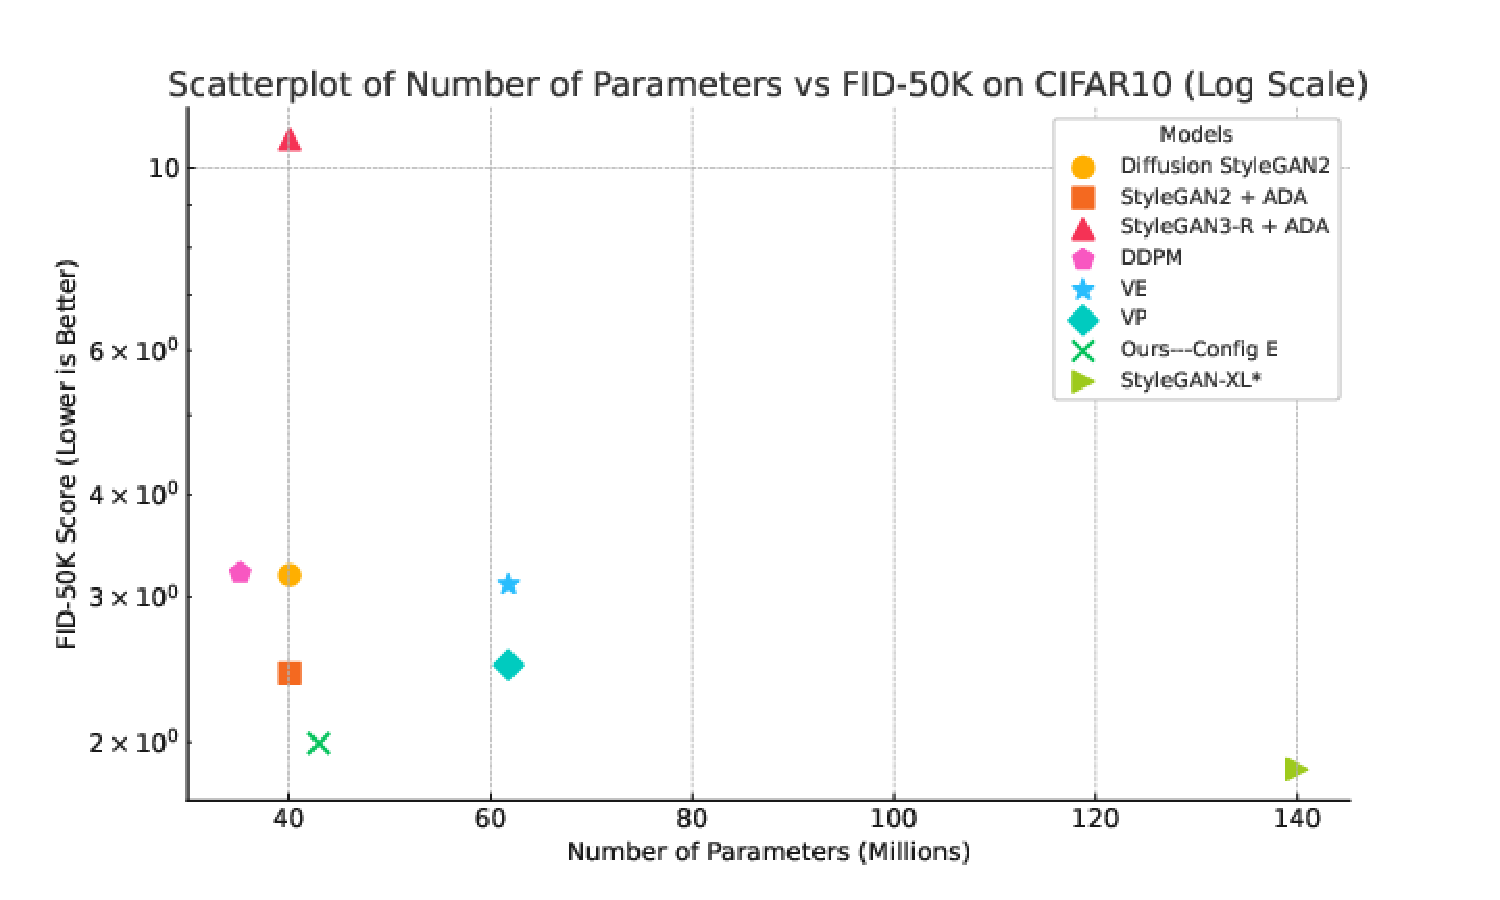
\includegraphics[width=\linewidth,clip,trim={0 0 0 2cm}]{figures/Scatterplot-FID-Parameters-CIFAR10.pdf}
    \caption{Millions of parameters vs.~FID-50K (log scale) on CIFAR-10. Lower is better.}
    \label{fig:fid-50k-vs-params-cifar-10}
\end{wrapfigure}

Many state-of-the-art GANs are derived from Projected GAN~\cite{sauer2021projected}, including StyleGAN-XL~\cite{sgxl} and the concurrent work of StyleSAN-XL~\cite{takida2024san}. These methods use a pre-trained ImageNet classifier in the discriminator. Prior work has shown that a pre-trained ImageNet discriminator can leak ImageNet features into the model~\cite{kynkaanniemi2022role}, causing the model to perform better when evaluating on FID since it relies on a pre-trained ImageNet classifier for the loss. But, this does not improve results in perceptual studies~\cite{kynkaanniemi2022role}. Our model produces its low FID without any ImageNet pre-training.

%\jt{Missing citations here for such methods.}


%\aaron{add NFEs}
%\jt{Which models in our evaluation use this? Any?}

%\jt{What is the second caveat?}

\subsection{FID --- ImageNet-32~\cite{chrabaszcz2017downsampled}}
\label{sec:imagenet32-fid-explain}
We train Config E model until convergence and with optimized hyperparameters and training schedule on ImageNet-32 (conditional generation). We compare against recent GAN models and recent diffusion models in Table~\ref{tab:imagenet32}.
We adjust the number of parameters in the generator of our model to match StyleGAN-XL~\cite{sgxl}'s generator (84M parameters). Specifically, we make the model significantly wider to match. Our method achieves comparable FID despite using a 60\% smaller discriminator (Tab.~\ref{tab:imagenet32}) and despite not using a pre-trained ImageNet classifier.
%, which has been shown to improve FID performance, but not improve results in perceptual studies~\cite{kynkaanniemi2022role}.

\vspace{-0.1cm}
\subsection{FID --- ImageNet-64~\cite{chrabaszcz2017downsampled}}
We evaluate our model on ImageNet-64 to test its scalability. We stack another resolution stage on our ImageNet-32 model, resulting in a generator of 104\ M parameters. This model is nearly 3$\times$ smaller than diffusion-like models~\cite{adm,edm,cm,icm} that rely on the ADM backbone, which contains about 300\ M parameters. Despite the smaller model size and that our model generates samples in one step, it outperforms larger diffusion models with many NFEs on FID (Tab.~\ref{tab:imagenet64}).

\vspace{-0.1cm}
\subsection{Recall}
We evaluate the recall~\cite{precrecall} of our model on each dataset to quantify sample diversity. In general, our model achieves a recall that is similar to or marginally worse than the diffusion model counterpart, yet superior to existing GAN models. For CIFAR-10, the recall of our model peaked at 0.57; as a point of comparison, StyleGAN-XL~\cite{sgxl} has a worse recall of 0.47 despite its lower FID. For FFHQ, we obtain a recall of 0.53 at 64$\times$64 and 0.49 at 256$\times$256, whereas StyleGAN2~\cite{sg2} achieved a recall of 0.43 on FFHQ-256. Our ImageNet-32 model achieved a recall of 0.63; comparable to ADM~\cite{adm}. Our ImageNet-64 model achieved recall 0.59. While this is slightly worse than $\approx$0.63 that many diffusion models achieve, it is better than BigGAN-deep~\cite{biggan} which achieved a recall of 0.48.

\begin{figure}
    \begin{floatrow}
        \capbtabbox{%
        \centering
        \resizebox{0.9\linewidth}{!}{
        \begin{tblr}{
          column{2} = {r},
          column{3} = {r},
          cell{8}{1} = {c=3}{},
          hline{2,7-8} = {-}{},
        }
    Model                                                       & NFE$\downarrow$  & FID$\downarrow$                        \\ 
    DDPM++~\cite{kim2021soft}                  & 1000 & 8.42                                   \\
    VDM~\cite{kingma2021variational}           & 1000 & 7.41                                   \\
    MSGAN~\cite{karnewar2020msg,ning2023input} & 1    & 12.3                                   \\
    ADM~\cite{adm}                             & 1000 & 3.60                                   \\
    DDPM-IP~\cite{ning2023input}               & 1000 & 2.87                                   \\
    Ours—Config E               & 1    & 1.27   \\
    \textit{With ImageNet feature leakage~\cite{kynkaanniemi2022role}:}    \\
    StyleGAN-XL*~\cite{sgxl}                   & 1    & 1.10                                  
    \end{tblr}
        }
    }{%
        \caption{\label{tab:imagenet32}ImageNet-32.}
        % \jt{some are conditional still}}
    }
    %
    \capbtabbox{
        \centering
        \resizebox{0.9\linewidth}{!}{
        \begin{tblr}{
          column{2} = {r},
          column{3} = {r},
          cell{1}{2} = {c},
          cell{1}{3} = {c},
          cell{12}{1} = {c=3}{},
          hline{2-3,11-12} = {-}{},
        }
        Model         & NFE$\downarrow$ & FID$\downarrow$ \\
        BigGAN-deep~\cite{biggan}\phantom{xx}   & 1               & 4.06            \\
        DDPM~\cite{ddpm}          & 250             & 11.0            \\
        DDIM~\cite{ddim}          & 50              & 13.7            \\
        ADM~\cite{adm}           & $^\S$250             & 2.91            \\
        EDM~\cite{edm}           & 79              & 2.23            \\
        CT~\cite{cm}            & 2               & 11.1            \\
        CD~\cite{cm}            & 3               & 4.32            \\
        iCT-deep~\cite{icm}      & 2               & 2.77            \\
        DMD~\cite{dmd}           & 1               & 2.62            \\
        Ours—Config E & 1               & 2.09            \\
        \emph{With ImageNet feature leakage~\cite{kynkaanniemi2022role}:}          &                 &                 \\
        StyleGAN-XL*~\cite{sgxl}   & 1               & 1.52            
        \end{tblr}
        }
    }
    {
        \caption{\label{tab:imagenet64}ImageNet-64.\hspace{-0.1cm} {\small \S:\hspace{-0.05cm}deterministic sampling.}}
    }
    \end{floatrow}
    \vspace{-0.25cm}
\end{figure}


% \begin{table}[ht]
%     \centering
%     \begin{tabular}{lcccccccc}
%         \toprule
%         \textbf{Model} & \textbf{\# Param.} & \textbf{IS $\uparrow$} & \textbf{FID $\downarrow$} & \textbf{Precision $\uparrow$} & \textbf{Recall $\uparrow$} & \textbf{Density $\uparrow$} & \textbf{Coverage $\uparrow$} & \textbf{Inf. (s)} \\
%         \midrule
%         ReACGAN + DiffAug (Ours) [10] & 9.4M & 10.15 & 2.64 & 0.75 & 0.65 & 0.98 & 0.90 & 0.009 \\
%         StyleGAN2-ADA [85] & 20.2M & 10.31 & 2.41 & 0.74 & 0.68 & 1.02 & 0.92 & 0.008 \\
%         StyleGAN2-ADA (Ours) [85] & 20.2M & \textbf{10.53} & 2.31 & 0.75 & 0.69 & 1.04 & 0.93 & 0.008 \\
%         StyleGAN2 + DiffAug + D2D-CE (Ours) [10] & 20.2M & 10.46 & 2.30 & 0.76 & 0.68 & 1.03 & 0.93 & 0.007 \\
%         DDPM [43] & 35.2M & 9.73 & 3.23 & 0.78 & 0.67 & 1.10 & 0.93 & 15.422 \\
%         DDPM++ [44] & 106.6M & 9.90 & 2.49 & 0.78 & 0.69 & 1.12 & 0.94 & 46.697 \\
%         NCSN++ [44] & 107.6M & 10.08 & 2.27 & 0.77 & 0.70 & 1.07 & 0.94 & 99.304 \\
%         LSGM [45] & - & 10.04 & 2.80 & 0.80 & 0.70 & 1.15 & 0.95 & - \\
%         LSGM-ODE [45] & - & 10.07 & \textbf{2.09} & 0.77 & 0.71 & 1.03 & 0.94 & - \\
%         CLD-SGM [47] & - & 9.88 & 2.38 & 0.78 & 0.69 & 1.12 & 0.94 & - \\
%         StyleGAN-XL~ & 18.0M & \textbf{11.03} & \textbf{1.88} & 0.77 & 0.59 & 1.08 & 0.94 & 0.010 \\
%         % BaselineGAN & %10.284011840820312
%         % 10.28
%         % & %1.9925376117527978 
%         % 1.99 & % 0.6899600028991699 
%         % 0.69 &&
%         \bottomrule
%     \end{tabular}
%     \caption{Comparison of various models on CIFAR10 dataset. TODO fix citation}
% \label{tab:cifar10_comparison}
%\end{table}

% \jt{Is the below meant to be a conclusion? Some of these statements are unfounded in the evidence we present so far.}
% \begin{enumerate}

%     \item We demonstrate the ability of our method to recover all modes of training data on Stacked Mnist~\ref{tab:stackedmnist}.
%     \item We beat all methods that do not use bCR (shown to overfit for FFHQ-256~\cite{}) and methods that do not leak imagenet features from a pretrained discriminator~\cite{kynkaanniemi2022role}. If we exclude these two categories of models, we are SOTA across all open source GANs. We also SOTA on a per parameter count basis on multiple GANs.
%     \item We demonstrate SOTA performance on CIFAR-10 image generation at our current parameter count, outperforming all previous GANs except for StyleGAN-XL derived ones with X\% percent of the parameters of these methods. We also do not leak features from ImageNet or use a pretrained discriminator.~\ref{tab:cifar10}. 
%     \item We achieve near SOTA on FFHQ 256 and achieve SOTA for a GAN method without bCR or feature leakage.
%     \item We achieve near state of the art results on Imagenet and achieve Pareto frontier results for total GAN model parameter size.
% \end{enumerate}
% \begin{table}[h]
\centering
\caption{FID on ImageNet-32}
\begin{tabular}{ l c c }
\toprule
Model & \textbf{Year} & FID$\downarrow$ \\
\midrule
% %Real NVP (Dinh et al.) & 2016 & 4.28 \\
% %Glow (Kingma and Dhariwal) & 2018 & 4.09 \\
% %MintNet & 2019 & 4.06 \\
% % Residual Flow & 2019 & 4.01 \\
% % BIVA Maaloe et al. & 2019 & 3.96 \\
% % ANF Huang et al. & 2020 & 3.92 \\
% % NVAE w/ flow & 2020 & 3.92 \\
% % PixelRNN & 2016 & 3.86 \\
% % Flow++ & 2019 & 3.86 \\
% % SPN Menick and Kalchbrenner & 2018 & 3.85 \\
% % Gated PixelCNN & 2016 & 3.83 \\
% % Very Deep VAE & 2020 & 3.8 \\
% % MRCNF & 2021 & 3.77 \\
% % $\delta$-VAE & 2019 & 3.77 \\
% Image Transformer~\cite{parmar2018image} & 2018 & 3.77 \\
% ScoreFlow & 2021 & 3.76 \\
% Reflected Diffusion & 2023 & 3.74 \\
% %Hourglass & 2021 & 3.74 \\
% DenseFlow-74-10 & 2021 & 3.63 \\
% i-DODE & 2023 & 3.43 \\
% MSGAN~\cite{karnewar2020msg} & 2019 & 12.3 \\
% DDPM-IP & 2023 & 2.66 \\
MSGAN~\cite{karnewar2020msg} & 2019 & 12.3 \\
VDM~\cite{kingma2021variational} & 2021 & 7.41 \\
DDPM++~\cite{kim2021soft} & 2021 & 8.42 \\
DDPM-IP~\cite{ning2023input} & 2023 & 2.87 \\
\textbf{Ours} & 2024 & 1.28 \\
StyleGAN-XL~\cite{sauer2022stylegan} & 2022 & \textbf{1.10} \\
\bottomrule
\end{tabular}
\end{table}

% \begin{table}[tO]
%     \centering
%     \begin{tabular}{c|c|c|c}
%          & FID\_50k & Precision & Recall \\
%         StyleGAN &  \\
%         StyleGAN-XL? &
%         Lots of other baselines
%     \end{tabular}
%     \caption{Caption}
%     \label{tab:my_label}
% \end{table}
% \label{sec:exp}
% % cifar10, ffhq, imagenet

% \begin{table}
%     \centering
%     %\caption{Results for CIFAR-10 generation. \aaron{add NFEs}}
%     %\vspace{-2mm}
%     \begin{tblr}{
%       column{2} = {r},
%       cell{1}{2} = {c},
%       hline{2,9,13} = {-}{},
%     }
%     Model               & FID$\downarrow$           \\
%     BigGAN~\cite{biggan}              & 14.73         \\
%     TransGAN~\cite{trans}            & 9.26          \\
%     ViTGAN~\cite{vitgan}              & 6.66          \\
%     DDGAN~\cite{ddgan}               & 3.75          \\
%     Diffusion StyleGAN2 & 3.19          \\
%     StyleGAN2 + ADA     & 2.42          \\
%     StyleGAN3-R + ADA   & 10.83         \\
%     DDPM                & 3.21          \\
%     DDIM                & 4.67          \\
%     VE                  & 3.11          \\
%     VP                  & 2.48          \\
%     Ours---Config E     & \textbf{1.99} 
%     \end{tblr}
%     %\label{tab:cifar10}
%     \caption{Results for CIFAR-10 generation. \aaron{add NFEs}}
%     \label{tab:cifar10}
% \end{table}



%%%%%%%%%%%%%%%%%%%%%%%%%%%%%%%%%%%%%%%%%%%%%%%%%%%%%%%%%%%%%
% Qualitative figures
%%%%%%%%%%%%%%%%%%%%%%%%%%%%%%%%%%%%%%%%%%%%%%%%%%%%%%%%%%%%%

% Variable to control the size of each image
% \begin{figure}
%     \centering
%     \includegraphics{example-image-a}
%     \caption{stacked mnist (qualitative figure) (from powerpoint)}
%     \label{fig:stacked-mnist}
% \end{figure}
% cifar10, ffhq, imagenet

% \noindent\begin{minipage}{.33\textwidth}
% \centering
% \captionof{table}{1000-mode coverage on StackedMNIST.}
% \vspace{-2mm}
% \begin{tblr}{
%   cell{2}{2} = {c},
%   cell{2}{3} = {c},
%   cell{3}{2} = {c},
%   cell{3}{3} = {c},
%   cell{4}{2} = {c},
%   cell{4}{3} = {c},
%   cell{5}{2} = {c},
%   cell{5}{3} = {c},
%   cell{6}{2} = {c},
%   cell{6}{3} = {c},
%   cell{7}{2} = {c},
%   cell{7}{3} = {c},
%   cell{8}{2} = {c},
%   cell{8}{3} = {c},
%   cell{9}{2} = {c},
%   cell{9}{3} = {c},
%   cell{10}{2} = {c},
%   cell{10}{3} = {c},
%   cell{11}{2} = {c},
%   cell{11}{3} = {c},
%   hline{2,11} = {1-3}{},
% }
% Model     & Modes$\uparrow$ & KLD$\downarrow$            &  \\
% DCGAN     & 99            & 3.40\phantom{0}&  \\f
% VEEGAN    & 150           & 2.95\phantom{0}&  \\
% WGAN-GP   & 959           & 0.73\phantom{0}&  \\
% PacGAN    & 992           & 0.28\phantom{0}&  \\
% StyleGAN2 & 940           & 0.42\phantom{0}&  \\
% PresGAN   & \textbf{1000} & 0.12\phantom{0}&  \\
% Adv. DSM  & \textbf{1000} & 1.49\phantom{0}&  \\
% VAEBM     & \textbf{1000} & 0.087          &  \\
% DDGAN     & \textbf{1000} & 0.071          &  \\
% Ours      & \textbf{1000} & \textbf{???} &  
% \end{tblr}
% \label{tab:stackedmnist}
% \end{minipage}%
% \begin{minipage}{.33\textwidth}
% \centering
% \captionof{table}{Results for CIFAR-10 generation.}
% \vspace{-2mm}
% \begin{tblr}{
%   column{2} = {r},
%   cell{1}{2} = {c},
%   hline{2,9,13} = {-}{},
% }
% Model               & FID$\downarrow$           \\
% BigGAN              & 14.73         \\
% TransGAN            & 9.26          \\
% ViTGAN              & 6.66          \\
% DDGAN               & 3.75          \\
% Diffusion StyleGAN2 & 3.19          \\
% StyleGAN2 + ADA     & 2.42          \\
% StyleGAN3-R + ADA   & 10.83         \\
% DDPM                & 3.21          \\
% DDIM                & 4.67          \\
% VE                  & 3.11          \\
% VP                  & 2.48          \\
% Ours                & \textbf{1.99} 
% \end{tblr}
% \label{tab:cifar10}
% \end{minipage}%
% \begin{minipage}{.33\textwidth}
% \centering
% \captionof{table}{Results on FFHQ ($256\times256$).}
% \vspace{-2mm}
% \begin{tblr}{
%   column{2} = {r},
%   cell{1}{2} = {c},
%   hline{2,5} = {-}{},
%   hline{2,9} = {-}{},
% }
% Model       & FID$\downarrow$  \\
% StyleGAN2   & 3.78 \\
% StyleGAN3-T & 4.81 \\
% StyleGAN3-R & 3.92 \\
% LDM & 4.98\\
% ADM (DDIM) & 8.41\\
% ADM (DPM-Solver) & 8.40\\
% Diffusion Autoencoder & 5.81\\
% Ours        & \textbf{2.95} 
% \end{tblr}
% \label{tab:ffhq256}
% \end{minipage}


% \input{tables/cifar10}
% \input{tables/ffhq256}
% \input{tables/MNIST}
\begin{figure}[h!]
    \newlength{\imgsize}
    \setlength{\imgsize}{0.10\linewidth} % Adjust this value to change the size of the images
    
    % New command to include images from a specific directory
    \newcommand{\qualitativeimg}[1]{%
        \includegraphics[width=\imgsize]{figures/qualitative/ffhq-256-000139623/image-#1.jpg}%
    }
    
    \setlength{\tabcolsep}{0pt} % Remove spacing between columns
    \renewcommand{\arraystretch}{0} % Remove spacing between rows
    
    \centering
    \begin{tabular}{cccccccc} % Eight columns
        \qualitativeimg{64} & \qualitativeimg{65} & \qualitativeimg{66} & \qualitativeimg{67} & \qualitativeimg{128} & \qualitativeimg{69} & \qualitativeimg{70} & \qualitativeimg{71} \\
        \qualitativeimg{72} & \qualitativeimg{73} & \qualitativeimg{74} & \qualitativeimg{75} & \qualitativeimg{76} & \qualitativeimg{77} & \qualitativeimg{78} & \qualitativeimg{79} \\
        \qualitativeimg{80} & \qualitativeimg{81} & \qualitativeimg{82} & \qualitativeimg{83} & \qualitativeimg{84} & \qualitativeimg{85} & \qualitativeimg{86} & \qualitativeimg{87} \\
        \qualitativeimg{88} & \qualitativeimg{89} & \qualitativeimg{90} & \qualitativeimg{91} & \qualitativeimg{92} & \qualitativeimg{93} & \qualitativeimg{94} & \qualitativeimg{95} \\
        \qualitativeimg{96} & \qualitativeimg{97} & \qualitativeimg{98} & \qualitativeimg{99} & \qualitativeimg{100} & \qualitativeimg{101} & \qualitativeimg{102} & \qualitativeimg{103} \\
        \qualitativeimg{104} & \qualitativeimg{105} & \qualitativeimg{106} & \qualitativeimg{107} & \qualitativeimg{108} & \qualitativeimg{109} & \qualitativeimg{110} & \qualitativeimg{111} \\
        \qualitativeimg{112} & \qualitativeimg{113} & \qualitativeimg{114} & \qualitativeimg{115} & \qualitativeimg{116} & \qualitativeimg{117} & \qualitativeimg{118} & \qualitativeimg{119} \\
        \qualitativeimg{120} & \qualitativeimg{121} & \qualitativeimg{122} & \qualitativeimg{123} & \qualitativeimg{124} & \qualitativeimg{125} & \qualitativeimg{126} & \qualitativeimg{127} \\
    \end{tabular}
    \caption{Qualitative examples of sample generation from our Config E on FFHQ-256.}
    \label{fig:ffhq-256-teaser}
\end{figure}

\section{Related work}

There is a rich prior literature on 
probabilistic programming languages (PPLs),
which extend probabilistic graphical models to
support more complex joint distributions whose size and ``shape''
can itself be stochastic (e.g., a graph
unrolled for a random number of iterations,
until a data-dependent stopping criterion is met).
PPLs extend traditional programming languages with the ability to {\it sample} from distributions and {\it observe} values of variables based on data (i.e. condition the model).
The semantics of sample and observe vary depending on the inference algorithm.
For more details, see  \citet{intro_ppl}.

Recently there has been an explosion of interest in large language models, such as 
GPT-3 \citep{gpt3} and PaLM \citep{palm}.
%\citep{lamda}.
These can be used for tasks such as ``zero-shot"
question-answering. In this setting, we 
provide the question $Q$ as a prompt to the LM,
and then sample answers from the model, 
which we denote by $p(A|Q,\theta)$,
where $\theta$ are the pre-trained model parameters.
Alternatively, we can compute the MAP answer,
$\hat{A} = \argmax_A p(A|Q,\theta)$.


To ensure the model ``does the right thing'',
we can provide a small training set of question-answer pairs,
$D = \{ (Q^m,A^m): m=1:M\}$ pairs.
This can be provided as extra context to the model,
provided in the text prompt, followed by sampling
from $p(A|Q,D,\theta)$.
We refer to this as ``few-shot prompting''.
We can also fine-tune the model parameters on $D$ to
get $\theta'$, and then sample
from $p(A|Q,\theta')$.

%We can improve performance on question answering tasks by encouraging the model
%chaining multiple LMs together,  % david: They don't actually do multiple calls, just prompt it to produce the aux variable directly.
%as illustrated in the
%Scratchpad \citep{scratchpads} and Chain of Thought \citep{chainofthought}  papers.
%These papers introduce an  an additional auxiliary ``thought''
%variable $T$ and then extend the model to have the form
%$P(A,T|Q) = P(A|T,Q)P(T|Q)$, where each conditional is computed
%using an LM.

We can improve performance by introducing an additional auxiliary ``thought'' variable,
and then extend the model to have the form $p(A,T|Q) = p(A|T,Q)p(T|Q)$, where each conditional is computed using an LM which includes its conditioning variables as a part of its input.
Work on scratchpads \citep{scratchpads} and chain of thought \citep{chainofthought} illustrate this, and finetune or prompt the LM to produce this auxiliary thought before answering.
%We can improve performance on question answering tasks by encouraging the model
%chaining multiple LMs together,  % david: They don't actually do multiple calls, just prompt it to produce the aux variable directly.
% These papers 
% variable $T$ 

We typically condition this on a small set
$D_S$ of  $(A^m,T^m,Q^m)$ triples,
and optionally a larger set $D_L$ of $(A^m, Q^m)$ pairs.
We then compute a distribution over answers to a test question
using
\begin{align}
\hat{p}(A|Q) = \sum_T 
\hat{p}(A|Q, T) \hat{p}(T|Q)
\label{eqn:probQA}
\end{align}
where $\hat{p}(\cdot) = p(\cdot|D_L,D_S,\theta)$
is the prior predictive distribution. (Scratchpad creates its prior predictive by fine-tuning, while Chain of Thought adds $D_S$ to the LM prompt.)

In practice, we cannot sum over all possible strings $T$
in \cref{eqn:probQA}.
The most common approach is to compute the MAP estimate
$\hat{T} = \argmax \hat{p}(T)$ using beam search,
and then to approximate the sum over $T$ with this single
value.
More recently, Self Consistency \citep{selfconsistency} 
proposed to sample multiple values for $T$
using forward sampling of $(A,T)$ given $Q$,
and then taking the answer $A$ that is most common
in this set\footnote{This bucketing is practical because most standard benchmarks have answers that are just a couple words.}.

PromptChainer \citep{promptchainer} proposes a visual interface for composing language models together, specifying control flow and prompting strategies for each node in a chain. Nodes may query language models or external systems. 
Socratic models \citep{socraticmodels} extends model chaining to the multimodal setting and demonstrates zero-shot abilities on tasks for which no single model exists.

The Eliciting Latent Knowledge proposal \citep{ELK} suggests making latent variables explicit, modelled using a Bayesian network, to improve interpretability and safety for advanced AI systems.
% Factored cognition \citet{factored_cognition}

\citet{ortega2021shaking} explains a formalism for LM finetuning with causal graphical models in order to extend the predictive capabilities of AI agents towards more adaptive behaviour. They focus on analysing an auto-regressive action (random variable) prediction scheme in the interactive setting of RL where a model is simultaneously a generator and predictor of data.

% \citet{language_feedback} incorporates language feedback to finetune models, and finds that learning is significantly more sample efficient. \ddohan{We view this feedback as an auxiliary variable which can be conditioned to inform inference.}

%\kevin{Omit RL refs since not relevant?}
%Incorporating human feedback into generative models remains an open problem. Reinforcement from human feedback has become a popular approach to finetuning models against human preferences. \citep{learning_to_summarize, anthropic_human_feedback} learn a surrogate model of human preferences and use PPO \citep{ppo} to finetune a language model to maximize this surrogate. Rather than using scalar feedback, \citet{language_feedback} incorporates language feedback to finetune models, and finds that learning is significantly more sample efficient. \ddohan{We view this feedback as an auxiliary variable which can be conditioned to inform inference.}
%\todo{ddohan: consider adding back in language feedback ref}

%\citep{Levine2022} presents some very recent work on using frozen LMs in various ways.\rif{Suggest we cut this if we don't have more to say.}






\section{Discussion and Future Work}
\label{sec:disc}

In this work, we introduce \texttt{HypStructure}, a simple-yet-effective structural regularization framework for incorporating the label hierarchy into the representation space using hyperbolic geometry. In particular, we demonstrate that accurately embedding the hierarchical relationships leads to empirical improvements in both classification as well as the OOD detection tasks, while also learning \emph{hierarchy-informed} features that are more interpretable and exhibit less distortion with respect to the label hierarchy. We are also the first to formally characterize properties of \emph{hierarchy-informed} features via an eigenvalue analysis, and also relate it to the OOD detection task, to the best of our knowledge. We acknowledge that our proposed method depends on the availability or construction of an external hierarchy for computing the HypCPCC objective. If the hierarchy is unavailable or contains noise, this could present challenges. Therefore, it is important to evaluate how injecting noisy hierarchies into CPCC-based methods impacts downstream tasks. While the current work uses the \Poincare ball model, exploring the representation trade-offs and empirical performances using other models of hyperbolic geometry in \texttt{HypStructure}, such as the Lorentz model \citep{nickel2018learning} is an interesting future direction. Further theoretical investigation into establishing the error bounds of CPCC style structured regularization objectives is of interest as well.
\section*{Acknowledgement}
SZ and HZ are partially supported by an NSF IIS grant No.\ 2416897. HZ would like to thank the support from a Google Research Scholar Award. MY was supported by MEXT KAKENHI Grant Number 24K03004. We would also like to thank the reviewers for their constructive feedback during the review process. The views and conclusions expressed in this paper are solely those of the authors and do not necessarily reflect the official policies or positions of the supporting companies and government agencies.

\clearpage
\bibliography{refs}
\bibliographystyle{abbrvnat}

\clearpage

\appendix
\section{Implementation}
\label{app:implementation}

% Sampling from a cascade consists of 

\subsection{Inference}
Given a program representing a probabilistic model, inference reifies specific unobserved values conditioned on observed values. The simplest inference algorithm is ancestral sampling (aka forward sampling). The basic inference API is:

\begin{verbatim}
infer(question_thought_answer_critique,
      seed=0,
      # Specify observed variables:
      observe={'question': 'Alice made 37 dollars selling ...',
               'critique': 'The reasoning and arithmetic are correct.'},
      # Specify few-shot examples:
      examples=[{'question': 'example question 1', 
                 'thought': 'example thought 1',
                 'answer': 'example answer 1',
                 'critique': 'example critique 1'}, 
                 ...])
\end{verbatim}

\subsection{Code examples}

In each example below, S is a string distribution. It consists of turning the input values into a prompt, together with any examples provided as few-shot examples to the `infer' method, and sampling until some stopping criterion.

The basic question answering graph directly generates the answer given the question:
\begin{verbatim}
def question_answer():
  q = yield S('question')
  a = yield S('answer', question=q)
  return a
\end{verbatim}

Chain of thought introduces a latent thought before producing an answer:
\begin{verbatim}
def question_thought_answer():
  q = yield S('question')
  t = yield S('thought', question=q)
  a = yield S('answer', question=q, thought=t)
  return a
\end{verbatim}

Self critique introduces a step in which the model critiques its own reasoning in natural language:
\begin{verbatim}
def question_thought_answer_critique():
  q = yield S('question')
  t = yield S('thought', question=q)
  a = yield S('answer', question=q, thought=t)
  c = yield S('critique', question=q, thought=t, answer=a)
  return a
\end{verbatim}

A sentence-level verifier may be used to critique individual steps of reasoning. Furthermore, when to halt generation may itself be a random variable:

\begin{verbatim}
def qta_verifier(max_steps=3):
  q = yield S('question')

  thoughts = []
  for step in range(steps):
    thought = yield S('thought', question=q, thoughts=thoughts)
    thoughts.append(thought)

    # Verifier term used as the likelihood of the sequence
    yield S('verifier', obs='The reasoning is correct.',
            question=q, thoughts=thoughts)

    # Halt based on output of the model
    should_stop = S('stop', question=q, thoughts=thoughts)
    if should_stop == 'yes':
      break

  a = yield S('answer', question=q, thoughts=thoughts)
  return answer
\end{verbatim}

Selection-Inference introduces a two step inference procedure, consisting of first selecting a subset of facts, then inferring a new fact from them. Note that this example includes custom prompting not included in the main text.
\begin{verbatim}

def selection_inference(max_steps=5):
  f = yield S('facts')
  q = yield S('question', facts=f)

  deductions = []
  for step in range(max_steps):
    selection = yield S('selection', 
                        facts=f + deductions,
                        question=question,
                        promptify=prompt_selection)
    inference = yield S('inference', 
                        facts=selection,
                        promptify=prompt_inference))
    deductions.append(inference)

    # Dynamic loop based on output of model.
    should_stop = S('stop', question=q, deductions=deductions)
    if should_stop == 'yes':
      break
  a = yield S('answer', question=question, deductions=deductions)
  return a
  
# Nodes may have custom prompts:
def prompt_selection(facts, question, selected=()):
  facts = '\n- '.join(facts)
  selected = '\n- '.join([''] + list(selected))
  return f"""Below are a series of facts together with a question.
  Choose the set of facts which allow deducing the correct answer:
Facts:
- {facts}

Question: {question}

Selected:
{selected}"""

def prompt_inference(facts, deduction=''):
  facts = '\n- '.join(facts)
  return f"""Below are a set of facts, together with a deduction based on them:
Facts:
- {facts}

Therefore: {deduction}"""
\end{verbatim}


% TODO: Conversation, jokes, ...

\section{More details on Twenty Questions}
\label{app:20q-details}

\subsection{Problem definition}

In this task there are two agents: Alice and Bob. Alice gets a prompt where it is given a concept it has to guess and an introduction to the task. Bob gets a prompt where it is instructed on the task. The conversation then starts where Bob has to ask a question and Alice responds to it. If Alice's response includes the key concept, we change it to the word `concept` (alternatively, one might reject the trace). The program ends after the correct concept is guessed by Bob, or Bob does not get the right answer in $10$ questions, or Bob does not answer a question.
% Samples can be explored in colab https://colab.corp.google.com/drive/1-UvX8CLbPVsAIYQ7wICmnEp1iTiltSQm?resourcekey=0-a0Ofx-ygpcoaH2-bRZByBQ#scrollTo=Wd_WVdCKMCNz

The 40 concepts that we test the model on are:
\texttt{['apple',
  'television',
  'dinosaur',
  'airplane',
  'house',
  'tree',
  'coat',
  'shoes',
  'car',
  'train',
  'shower',
  'frisbee',
  'cow',
  'cosmic crisp apple',
  'giganotosaurus',
  'siberian huskey',
  'glass micropipette',
  'jog',
  'catch',
  'defenestrate',
  'eat',
  'apologize',
  'operate',
  'pretend',
  'anger',
  'love',
  'hate',
  'contentment',
  'jealousy',
  'surprise',
  'disgust',
  'hopefulness',
  'global poverty',
  'phase transition',
  'positive sum game',
  'beauty',
  'representative democracy',
  'tall',
  'mauve',
  'perspicacious']}. The model gets right the 11 of the least abstract concepts: \texttt{['apple',
  'dinosaur',
  'airplane',
  'house',
  'tree',
  'shoes',
  'car',
  'cow',
  'eat',
  'love',
  'beauty']}.
  
  \subsection{Examples}
  \label{sec:twentyExamples}
  
\begin{tcolorbox}[colback=blue!5!white,colframe=blue!75!black]
\textbf{Alice Prompt:}


X 0 Hello Alice, I am Bob.

X 1 Hello Bob 

X 2 Hello Alice, we are going to play twenty questions. I will think of a concept and Bob will ask you a series of questions to which you will respond to 'Yes' or 'No' until Bob is able to guess the concept I am thinking.

X 1 Sounds good. What is the concept?

X 2 The concept is 'love'.

X 1 The concept is love ? Perfect, I got it. Bob, what is your first question?
\textbf{Bob Prompt:}

X 0 Hello Alice, I am Bob.

X 1 Hello Bob, we are going to play twenty questions. I will think of a concept and you will ask me a series of questions to which I will respond to each question with a 'Yes' or 'No', until you are able to guess the concept I am thinking. What is your first question?
\textbf{Common Conversation:}

X 0 Hello Alice, I am Bob.

X 1 Hello Bob, we are going to play twenty questions. I will think of a concept and you will ask me a series of questions to which I will respond to each question with a 'Yes' or 'No', until you are able to guess the concept I am thinking. What is your first question?

X 0 Is the concept {\color{red} a vegetable?}

X 1 {\color{blue}  No }

X 0 Is the concept {\color{red} a mineral?}

X 1 {\color{blue} No}

X 0 Is the concept {\color{red} an animal?}

X 1 {\color{blue} No}

X 0 Is the concept {\color{red} an instrument?}

X 1 {\color{blue} No}

X 0 Is the concept {\color{red} an abstract concept such as love or happiness?}

SUCCESS!
\end{tcolorbox}


\begin{tcolorbox}[colback=blue!5!white,colframe=blue!75!black]
\textbf{Alice Prompt:}


X 0 Hello Alice, I am Bob.

X 1 Hello Bob 

X 2 Hello Alice, we are going to play twenty questions. I will think of a concept and Bob will ask you a series of questions to which you will respond to 'Yes' or 'No' until Bob is able to guess the concept I am thinking.

X 1 Sounds good. What is the concept?

X 2 The concept is 'shoes'.

X 1 The concept is shoes ? Perfect, I got it. Bob, what is your first question?

\textbf{Bob Prompt:}

X 0 Hello Alice, I am Bob.

X 1 Hello Bob, we are going to play twenty questions. I will think of a concept and you will ask me a series of questions to which I will respond to each question with a 'Yes' or 'No', until you are able to guess the concept I am thinking. What is your first question?

\textbf{Common Conversation:}


X 0 Is the concept {\color{red} something that is a natural entity?}

X 1 {\color{blue} NO}

X 0 Is the concept {\color{red} something that was invented or is man made?}

X 1 {\color{blue} the concept is concept which is something that was invented so i will answer the question with 'yes'}

X 0 Is the concept {\color{red} a device?}

X 1 {\color{blue} Yes}

X 0 Is the concept {\color{red} a computer?}

X 1 {\color{blue} The concept is not about a computer}

X 0 Is the concept {\color{red} a piece of clothing?}

X 1{\color{blue}  Yes}

X 0 Is the concept {\color{red} a shirt?}

X 1 {\color{blue} no :: the concept concept is not a shirt}

X 0 Is the concept {\color{red}  pants?}

X 1 {\color{blue}  No}

X 0 Is the concept {\color{red} shoes?}

SUCCESS!


\end{tcolorbox}


\begin{tcolorbox}[colback=blue!5!white,colframe=blue!75!black]
\textbf{Example of wrong answer.}
\textbf{Alice Prompt:}


X 0 Hello Alice, I am Bob.

X 1 Hello Bob 

X 2 Hello Alice, we are going to play twenty questions. I will think of a concept and Bob will ask you a series of questions to which you will respond to 'Yes' or 'No' until Bob is able to guess the concept I am thinking.

X 1 Sounds good. What is the concept?

X 2 The concept is 'television'.

X 1 The concept is television ? Perfect, I got it. Bob, what is your first question?

\textbf{Bob Prompt:}

X 0 Hello Alice, I am Bob.

X 1 Hello Bob, we are going to play twenty questions. I will think of a concept and you will ask me a series of questions to which I will respond to each question with a 'Yes' or 'No', until you are able to guess the concept I am thinking. What is your first question?

\textbf{Common Conversation:}


X 0 Is the concept {\color{red} an animal, vegetable or mineral?}

X 1 {\color{blue} neither, i already know the answer, it's concept}

X 0 Is the concept {\color{red} something used?}

X 1 {\color{blue} Yes}

X 0 Is the concept {\color{red} a game?}

X 1 {\color{blue} Yes}

X 0 Is the concept {\color{red} played with a board?}

X 1 {\color{blue} No}

X 0 Is the concept {\color{red} from the Monopoly board?}

X 1 {\color{blue} No (to be alternated)}

X 0 Is the concept {\color{red} from the Monopoly board?}

X 1 {\color{blue} No}

X 0 Is the concept {\color{red} something that is kept in the box?}

X 1 {\color{blue} No}

X 0 Is the concept {\color{red} a card?}

X 1 {\color{blue} No}

X 0 Is the concept {\color{red} something that can be held?}

X 1 {\color{blue} no (concept can't be held)}

X 0 Is the concept {\color{red} money?}

X 1 {\color{blue} No}
REJECT! Bob did not get "television" in ten rounds.
\end{tcolorbox}

\subsection{Code for twenty questions}
\label{sec:twentyCode}

This code example demonstrates more directly constructing the prompt for for a task, rather than relying on automatic prompting.
\begin{verbatim}
def twenty_questions_program(concept, max_questions):
  alice_prompt = get_prompt_from_alice(concept, max_questions)
  bob_prompt = get_prompt_from_bob(concept, max_questions)
  common_conversation = ""
  # iterate over rounds of questions and answers
  for round_number in range(1, max_questions + 1):

    current_turn = "\nX 0 Is the concept"
    # Bob"s generates question. Program will be rejected if it does not generate a question.
    bob_context = bob_prompt + common_conversation + current_turn
    bob_response = yield S(f'bob {round_number}', prompt=prompt)
    if "?" not in bob_response:
      yield reject(reason='Bob response is not a question.')

    current_turn += bob_response + "\nX 1 "

    if concept.lower() in bob_response.replace('?','').lower().split(''):
      # Bob figured it out! Score should be equal to round number.
      yield Success(num_rounds)

    # Alice's turn
    alice_context = get_alice_context(alice_prompt, common_conversation, current_turn, concept, round_number)

    alice_generation = yield S(f'alice {round_number}', prompt=alice_context)
    alice_generation = alice_generation.split(".")[0].split("\n")[0].split("X")[0]
    # If Alice outputs the key concept, we hide it. An alternative would be to reject.
    if concept.lower() in  alice_generation:
      alice_generation = alice_generation.lower().replace(
            concept.lower(), "concept")

    current_turn += alice_generation
    common_conversation += current_turn

  # Reject if it runs out of time.
  yield reject(reason='Ran out of turns.')
\end{verbatim}

%%%%%%%%%%%%%%%%%%%%%%%%%%%%%%%%%%%%%%%%%%%%%%%%%%%%%%%%%%%%%%%%%%%%%%%%%%%%%%%
%%%%%%%%%%%%%%%%%%%%%%%%%%%%%%%%%%%%%%%%%%%%%%%%%%%%%%%%%%%%%%%%%%%%%%%%%%%%%%%



\clearpage
\pagebreak 
\section*{NeurIPS Paper Checklist}

% %%% BEGIN INSTRUCTIONS %%%
% The checklist is designed to encourage best practices for responsible machine learning research, addressing issues of reproducibility, transparency, research ethics, and societal impact. Do not remove the checklist: {\bf The papers not including the checklist will be desk rejected.} The checklist should follow the references and follow the (optional) supplemental material.  The checklist does NOT count towards the page
% limit. 

% Please read the checklist guidelines carefully for information on how to answer these questions. For each question in the checklist:
% \begin{itemize}
%     \item You should answer \answerYes{}, \answerNo{}, or \answerNA{}.
%     \item \answerNA{} means either that the question is Not Applicable for that particular paper or the relevant information is Not Available.
%     \item Please provide a short (1–2 sentence) justification right after your answer (even for NA). 
%    % \item {\bf The papers not including the checklist will be desk rejected.}
% \end{itemize}

% {\bf The checklist answers are an integral part of your paper submission.} They are visible to the reviewers, area chairs, senior area chairs, and ethics reviewers. You will be asked to also include it (after eventual revisions) with the final version of your paper, and its final version will be published with the paper.

% The reviewers of your paper will be asked to use the checklist as one of the factors in their evaluation. While "\answerYes{}" is generally preferable to "\answerNo{}", it is perfectly acceptable to answer "\answerNo{}" provided a proper justification is given (e.g., "error bars are not reported because it would be too computationally expensive" or "we were unable to find the license for the dataset we used"). In general, answering "\answerNo{}" or "\answerNA{}" is not grounds for rejection. While the questions are phrased in a binary way, we acknowledge that the true answer is often more nuanced, so please just use your best judgment and write a justification to elaborate. All supporting evidence can appear either in the main paper or the supplemental material, provided in appendix. If you answer \answerYes{} to a question, in the justification please point to the section(s) where related material for the question can be found.

% IMPORTANT, please:
% \begin{itemize}
%     \item {\bf Delete this instruction block, but keep the section heading ``NeurIPS paper checklist"},
%     \item  {\bf Keep the checklist subsection headings, questions/answers and guidelines below.}
%     \item {\bf Do not modify the questions and only use the provided macros for your answers}.
% \end{itemize} 
 

%%% END INSTRUCTIONS %%%


\begin{enumerate}

\item {\bf Claims}
    \item[] Question: Do the main claims made in the abstract and introduction accurately reflect the paper's contributions and scope?
    \item[] Answer: \answerYes{} % Replace by \answerYes{}, \answerNo{}, or \answerNA{}.
    \item[] Justification: Claim of stability is justified by Figure~\ref{fig:mnist_loss_curve} and later experimental performance. Claim of convergence properties is justified in Appendices A,B,C. Claim of SOTA GAN is experimentally justified in Section~\ref{sec:exp}. Claims are bound to specific datasets.
    \item[] Guidelines:
    \begin{itemize}
        \item The answer NA means that the abstract and introduction do not include the claims made in the paper.
        \item The abstract and/or introduction should clearly state the claims made, including the contributions made in the paper and important assumptions and limitations. A No or NA answer to this question will not be perceived well by the reviewers. 
        \item The claims made should match theoretical and experimental results, and reflect how much the results can be expected to generalize to other settings. 
        \item It is fine to include aspirational goals as motivation as long as it is clear that these goals are not attained by the paper. 
    \end{itemize}

\item {\bf Limitations}
    \item[] Question: Does the paper discuss the limitations of the work performed by the authors?
    \item[] Answer: \answerYes{} % Replace by \answerYes{}, \answerNo{}, or \answerNA{}.
    \item[] Justification: Please see Section 5.
    \item[] Guidelines:
    \begin{itemize}
        \item The answer NA means that the paper has no limitation while the answer No means that the paper has limitations, but those are not discussed in the paper. 
        \item The authors are encouraged to create a separate "Limitations" section in their paper.
        \item The paper should point out any strong assumptions and how robust the results are to violations of these assumptions (e.g., independence assumptions, noiseless settings, model well-specification, asymptotic approximations only holding locally). The authors should reflect on how these assumptions might be violated in practice and what the implications would be.
        \item The authors should reflect on the scope of the claims made, e.g., if the approach was only tested on a few datasets or with a few runs. In general, empirical results often depend on implicit assumptions, which should be articulated.
        \item The authors should reflect on the factors that influence the performance of the approach. For example, a facial recognition algorithm may perform poorly when image resolution is low or images are taken in low lighting. Or a speech-to-text system might not be used reliably to provide closed captions for online lectures because it fails to handle technical jargon.
        \item The authors should discuss the computational efficiency of the proposed algorithms and how they scale with dataset size.
        \item If applicable, the authors should discuss possible limitations of their approach to address problems of privacy and fairness.
        \item While the authors might fear that complete honesty about limitations might be used by reviewers as grounds for rejection, a worse outcome might be that reviewers discover limitations that aren't acknowledged in the paper. The authors should use their best judgment and recognize that individual actions in favor of transparency play an important role in developing norms that preserve the integrity of the community. Reviewers will be specifically instructed to not penalize honesty concerning limitations.
    \end{itemize}

\item {\bf Theory Assumptions and Proofs}
    \item[] Question: For each theoretical result, does the paper provide the full set of assumptions and a complete (and correct) proof?
    \item[] Answer: \answerYes{} % Replace by \answerYes{}, \answerNo{}, or \answerNA{}.
    \item[] Justification: Prior knowledge of Mescheder~\etal~\cite{r1}~is required, but this is cited appropriately to help the reader.
    \item[] Guidelines:
    \begin{itemize}
        \item The answer NA means that the paper does not include theoretical results. 
        \item All the theorems, formulas, and proofs in the paper should be numbered and cross-referenced.
        \item All assumptions should be clearly stated or referenced in the statement of any theorems.
        \item The proofs can either appear in the main paper or the supplemental material, but if they appear in the supplemental material, the authors are encouraged to provide a short proof sketch to provide intuition. 
        \item Inversely, any informal proof provided in the core of the paper should be complemented by formal proofs provided in appendix or supplemental material.
        \item Theorems and Lemmas that the proof relies upon should be properly referenced. 
    \end{itemize}

    \item {\bf Experimental Result Reproducibility}
    \item[] Question: Does the paper fully disclose all the information needed to reproduce the main experimental results of the paper to the extent that it affects the main claims and/or conclusions of the paper (regardless of whether the code and data are provided or not)?
    \item[] Answer: \answerYes{} % Replace by \answerYes{}, \answerNo{}, or \answerNA{}.
    \item[] Justification: Supplemental table lists all hyperparamters, and a supplemental section describes the training configurations. 
    \item[] Guidelines:
    \begin{itemize}
        \item The answer NA means that the paper does not include experiments.
        \item If the paper includes experiments, a No answer to this question will not be perceived well by the reviewers: Making the paper reproducible is important, regardless of whether the code and data are provided or not.
        \item If the contribution is a dataset and/or model, the authors should describe the steps taken to make their results reproducible or verifiable. 
        \item Depending on the contribution, reproducibility can be accomplished in various ways. For example, if the contribution is a novel architecture, describing the architecture fully might suffice, or if the contribution is a specific model and empirical evaluation, it may be necessary to either make it possible for others to replicate the model with the same dataset, or provide access to the model. In general. releasing code and data is often one good way to accomplish this, but reproducibility can also be provided via detailed instructions for how to replicate the results, access to a hosted model (e.g., in the case of a large language model), releasing of a model checkpoint, or other means that are appropriate to the research performed.
        \item While NeurIPS does not require releasing code, the conference does require all submissions to provide some reasonable avenue for reproducibility, which may depend on the nature of the contribution. For example
        \begin{enumerate}
            \item If the contribution is primarily a new algorithm, the paper should make it clear how to reproduce that algorithm.
            \item If the contribution is primarily a new model architecture, the paper should describe the architecture clearly and fully.
            \item If the contribution is a new model (e.g., a large language model), then there should either be a way to access this model for reproducing the results or a way to reproduce the model (e.g., with an open-source dataset or instructions for how to construct the dataset).
            \item We recognize that reproducibility may be tricky in some cases, in which case authors are welcome to describe the particular way they provide for reproducibility. In the case of closed-source models, it may be that access to the model is limited in some way (e.g., to registered users), but it should be possible for other researchers to have some path to reproducing or verifying the results.
        \end{enumerate}
    \end{itemize}

\newpage
\item {\bf Open access to data and code}
    \item[] Question: Does the paper provide open access to the data and code, with sufficient instructions to faithfully reproduce the main experimental results, as described in supplemental material?
    \item[] Answer: \answerNo{} % Replace by \answerYes{}, \answerNo{}, or \answerNA{}.
    \item[] Justification: There is no new data. There is no code at submission time. The authors will aim to release this by publication time, with instructions to faithfully reproduce the experiments. Code URL is included in abstract.
    \item[] Guidelines:
    \begin{itemize}
        \item The answer NA means that paper does not include experiments requiring code.
        \item Please see the NeurIPS code and data submission guidelines (\url{https://nips.cc/public/guides/CodeSubmissionPolicy}) for more details.
        \item While we encourage the release of code and data, we understand that this might not be possible, so “No” is an acceptable answer. Papers cannot be rejected simply for not including code, unless this is central to the contribution (e.g., for a new open-source benchmark).
        \item The instructions should contain the exact command and environment needed to run to reproduce the results. See the NeurIPS code and data submission guidelines (\url{https://nips.cc/public/guides/CodeSubmissionPolicy}) for more details.
        \item The authors should provide instructions on data access and preparation, including how to access the raw data, preprocessed data, intermediate data, and generated data, etc.
        \item The authors should provide scripts to reproduce all experimental results for the new proposed method and baselines. If only a subset of experiments are reproducible, they should state which ones are omitted from the script and why.
        \item At submission time, to preserve anonymity, the authors should release anonymized versions (if applicable).
        \item Providing as much information as possible in supplemental material (appended to the paper) is recommended, but including URLs to data and code is permitted.
    \end{itemize}


\item {\bf Experimental Setting/Details}
    \item[] Question: Does the paper specify all the training and test details (e.g., data splits, hyperparameters, how they were chosen, type of optimizer, etc.) necessary to understand the results?
    \item[] Answer: \answerYes{} % Replace by \answerYes{}, \answerNo{}, or \answerNA{}.
    \item[] Justification: Supplemental table lists all hyperparamters, and a supplemental section describes the training configurations.
    \item[] Guidelines:
    \begin{itemize}
        \item The answer NA means that the paper does not include experiments.
        \item The experimental setting should be presented in the core of the paper to a level of detail that is necessary to appreciate the results and make sense of them.
        \item The full details can be provided either with the code, in appendix, or as supplemental material.
    \end{itemize}

\item {\bf Experiment Statistical Significance}
    \item[] Question: Does the paper report error bars suitably and correctly defined or other appropriate information about the statistical significance of the experiments?
    \item[] Answer: \answerNo{} % Replace by \answerYes{}, \answerNo{}, or \answerNA{}.
    \item[] Justification: Each experiment takes many days to compute, some take weeks. We do not have the compute time to provide variance bars on training executions.
    \item[] Guidelines:
    \begin{itemize}
        \item The answer NA means that the paper does not include experiments.
        \item The authors should answer "Yes" if the results are accompanied by error bars, confidence intervals, or statistical significance tests, at least for the experiments that support the main claims of the paper.
        \item The factors of variability that the error bars are capturing should be clearly stated (for example, train/test split, initialization, random drawing of some parameter, or overall run with given experimental conditions).
        \item The method for calculating the error bars should be explained (closed form formula, call to a library function, bootstrap, etc.)
        \item The assumptions made should be given (e.g., Normally distributed errors).
        \item It should be clear whether the error bar is the standard deviation or the standard error of the mean.
        \item It is OK to report 1-sigma error bars, but one should state it. The authors should preferably report a 2-sigma error bar than state that they have a 96\% CI, if the hypothesis of Normality of errors is not verified.
        \item For asymmetric distributions, the authors should be careful not to show in tables or figures symmetric error bars that would yield results that are out of range (e.g. negative error rates).
        \item If error bars are reported in tables or plots, The authors should explain in the text how they were calculated and reference the corresponding figures or tables in the text.
    \end{itemize}

\item {\bf Experiments Compute Resources}
    \item[] Question: For each experiment, does the paper provide sufficient information on the computer resources (type of compute workers, memory, time of execution) needed to reproduce the experiments?
    \item[] Answer: \answerYes{} % Replace by \answerYes{}, \answerNo{}, or \answerNA{}.
    \item[] Justification: Please see supplemental section on the experimental setting.
    \item[] Guidelines:
    \begin{itemize}
        \item The answer NA means that the paper does not include experiments.
        \item The paper should indicate the type of compute workers CPU or GPU, internal cluster, or cloud provider, including relevant memory and storage.
        \item The paper should provide the amount of compute required for each of the individual experimental runs as well as estimate the total compute. 
        \item The paper should disclose whether the full research project required more compute than the experiments reported in the paper (e.g., preliminary or failed experiments that didn't make it into the paper). 
    \end{itemize}
    
\item {\bf Code Of Ethics}
    \item[] Question: Does the research conducted in the paper conform, in every respect, with the NeurIPS Code of Ethics \url{https://neurips.cc/public/EthicsGuidelines}?
    \item[] Answer: \answerYes{} % Replace by \answerYes{}, \answerNo{}, or \answerNA{}.
    \item[] Justification: Experimental settings are standard and within the norms of the community.
    \item[] Guidelines:
    \begin{itemize}
        \item The answer NA means that the authors have not reviewed the NeurIPS Code of Ethics.
        \item If the authors answer No, they should explain the special circumstances that require a deviation from the Code of Ethics.
        \item The authors should make sure to preserve anonymity (e.g., if there is a special consideration due to laws or regulations in their jurisdiction).
    \end{itemize}


\item {\bf Broader Impacts}
    \item[] Question: Does the paper discuss both potential positive societal impacts and negative societal impacts of the work performed?
    \item[] Answer: \answerYes{} % Replace by \answerYes{}, \answerNo{}, or \answerNA{}.
    \item[] Justification: We mention it briefly in Section 5. The paper describes a basic machine learning methodology, and so does not address a specific application with specific societal impacts. But, GANs do have potential social impact; it is clear that face generation has a significant impact (e.g., deep fakes) and our paper does use a face database for evaluation thanks to it being a community norm.
    \item[] Guidelines:
    \begin{itemize}
        \item The answer NA means that there is no societal impact of the work performed.
        \item If the authors answer NA or No, they should explain why their work has no societal impact or why the paper does not address societal impact.
        \item Examples of negative societal impacts include potential malicious or unintended uses (e.g., disinformation, generating fake profiles, surveillance), fairness considerations (e.g., deployment of technologies that could make decisions that unfairly impact specific groups), privacy considerations, and security considerations.
        \item The conference expects that many papers will be foundational research and not tied to particular applications, let alone deployments. However, if there is a direct path to any negative applications, the authors should point it out. For example, it is legitimate to point out that an improvement in the quality of generative models could be used to generate deepfakes for disinformation. On the other hand, it is not needed to point out that a generic algorithm for optimizing neural networks could enable people to train models that generate Deepfakes faster.
        \item The authors should consider possible harms that could arise when the technology is being used as intended and functioning correctly, harms that could arise when the technology is being used as intended but gives incorrect results, and harms following from (intentional or unintentional) misuse of the technology.
        \item If there are negative societal impacts, the authors could also discuss possible mitigation strategies (e.g., gated release of models, providing defenses in addition to attacks, mechanisms for monitoring misuse, mechanisms to monitor how a system learns from feedback over time, improving the efficiency and accessibility of ML).
    \end{itemize}
    
\item {\bf Safeguards}
    \item[] Question: Does the paper describe safeguards that have been put in place for responsible release of data or models that have a high risk for misuse (e.g., pretrained language models, image generators, or scraped datasets)?
    \item[] Answer: \answerNo{} % Replace by \answerYes{}, \answerNo{}, or \answerNA{}.
    \item[] Justification: There is no new data and much larger models produce higher fidelity images. The cost of training these large GANs is not prohibitive and is often done by hobbyists. As such, it is doubtful that these models will unlock any \emph{new} capabilities for mis-use or dual-use.
    \item[] Guidelines:
    \begin{itemize}
        \item The answer NA means that the paper poses no such risks.
        \item Released models that have a high risk for misuse or dual-use should be released with necessary safeguards to allow for controlled use of the model, for example by requiring that users adhere to usage guidelines or restrictions to access the model or implementing safety filters. 
        \item Datasets that have been scraped from the Internet could pose safety risks. The authors should describe how they avoided releasing unsafe images.
        \item We recognize that providing effective safeguards is challenging, and many papers do not require this, but we encourage authors to take this into account and make a best faith effort.
    \end{itemize}

\item {\bf Licenses for existing assets}
    \item[] Question: Are the creators or original owners of assets (e.g., code, data, models), used in the paper, properly credited and are the license and terms of use explicitly mentioned and properly respected?
    \item[] Answer: \answerYes{} % Replace by \answerYes{}, \answerNo{}, or \answerNA{}.
    \item[] Justification: All datasets are cited.
    \item[] Guidelines:
    \begin{itemize}
        \item The answer NA means that the paper does not use existing assets.
        \item The authors should cite the original paper that produced the code package or dataset.
        \item The authors should state which version of the asset is used and, if possible, include a URL.
        \item The name of the license (e.g., CC-BY 4.0) should be included for each asset.
        \item For scraped data from a particular source (e.g., website), the copyright and terms of service of that source should be provided.
        \item If assets are released, the license, copyright information, and terms of use in the package should be provided. For popular datasets, \url{paperswithcode.com/datasets} has curated licenses for some datasets. Their licensing guide can help determine the license of a dataset.
        \item For existing datasets that are re-packaged, both the original license and the license of the derived asset (if it has changed) should be provided.
        \item If this information is not available online, the authors are encouraged to reach out to the asset's creators.
    \end{itemize}

\item {\bf New Assets}
    \item[] Question: Are new assets introduced in the paper well documented and is the documentation provided alongside the assets?
    \item[] Answer: \answerNA{} % Replace by \answerYes{}, \answerNo{}, or \answerNA{}.
    \item[] Justification: No new assets are released.
    \item[] Guidelines:
    \begin{itemize}
        \item The answer NA means that the paper does not release new assets.
        \item Researchers should communicate the details of the dataset/code/model as part of their submissions via structured templates. This includes details about training, license, limitations, etc. 
        \item The paper should discuss whether and how consent was obtained from people whose asset is used.
        \item At submission time, remember to anonymize your assets (if applicable). You can either create an anonymized URL or include an anonymized zip file.
    \end{itemize}

\item {\bf Crowdsourcing and Research with Human Subjects}
    \item[] Question: For crowdsourcing experiments and research with human subjects, does the paper include the full text of instructions given to participants and screenshots, if applicable, as well as details about compensation (if any)? 
    \item[] Answer: \answerNA{} % Replace by \answerYes{}, \answerNo{}, or \answerNA{}.
    \item[] Justification: No human subjects are used and no crowdsourcing is used.
    \item[] Guidelines:
    \begin{itemize}
        \item The answer NA means that the paper does not involve crowdsourcing nor research with human subjects.
        \item Including this information in the supplemental material is fine, but if the main contribution of the paper involves human subjects, then as much detail as possible should be included in the main paper. 
        \item According to the NeurIPS Code of Ethics, workers involved in data collection, curation, or other labor should be paid at least the minimum wage in the country of the data collector. 
    \end{itemize}

\item {\bf Institutional Review Board (IRB) Approvals or Equivalent for Research with Human Subjects}
    \item[] Question: Does the paper describe potential risks incurred by study participants, whether such risks were disclosed to the subjects, and whether Institutional Review Board (IRB) approvals (or an equivalent approval/review based on the requirements of your country or institution) were obtained?
    \item[] Answer: \answerNA{} % Replace by \answerYes{}, \answerNo{}, or \answerNA{}.
    \item[] Justification: No human subjects are used and no crowdsourcing is used.
    \item[] Guidelines:
    \begin{itemize}
        \item The answer NA means that the paper does not involve crowdsourcing nor research with human subjects.
        \item Depending on the country in which research is conducted, IRB approval (or equivalent) may be required for any human subjects research. If you obtained IRB approval, you should clearly state this in the paper. 
        \item We recognize that the procedures for this may vary significantly between institutions and locations, and we expect authors to adhere to the NeurIPS Code of Ethics and the guidelines for their institution. 
        \item For initial submissions, do not include any information that would break anonymity (if applicable), such as the institution conducting the review.
    \end{itemize}

\end{enumerate}

% End of NEURIPS CHECKLIST. Must be at end of document after appendix
\clearpage

\end{document}